\chapter{WebRTC 专家策略数据集采集和构建}
\label{chap:dataset_construction}

离线强化学习的策略性能上限完全由训练数据集的质量与覆盖度决定。本章围绕 WebRTC 拥塞控制任务，论述专家策略数据集的采集、预处理与离线强化学习四元组的构建方法。本章首先介绍承担数据采集与策略部署验证双重职责的实验平台总体架构；其次，分析端到端数据采集链路的工程实现；进而阐述以 Google Congestion Control（GCC）作为专家行为策略所收集的原始网络轨迹及其多阶段清洗流程；最后，给出从清洗后轨迹到标准化 $(s_t, a_t, r_t, s_{t+1})$ 四元组数据集的完整构建过程。

\section{实验平台总体架构设计}
\label{sec:platform-architecture}

为打破现有 RTC 拥塞控制研究中“在线探索风险高、纯仿真失真大”的困境，本文构建了一套基于真实物理信道的端到端实验平台。平台遵循数据采集与部署评测严格隔离的设计准则，将系统划分为四个相互解耦的组件：负责采集真实链路状态的网络轨迹采集模块、承担特征工程与策略训练的算法模块、用于在线对照实验的 A/B 测试模块，以及通过流量整形工具构造可控信道条件的网络控制模块。各模块在端口与文件系统层面相互隔离，从根本上杜绝了数据采集阶段与策略评测阶段的互相影响。

平台的端到端架构遵循“感知—决策—反馈”的控制路径。在客户端侧，浏览器内置的 WebRTC 引擎承担媒体数据流的捕获、编码与传输；控制平面通过周期性调用 \texttt{getStats()} 接口获取实时链路状态，将状态向量送入策略中心（本地/后端模型）；策略中心输出的目标码率指令经由 \texttt{RTCRtpSender.setParameters()} 注入媒体发送链路，完成对底层码率的控制。平台整体拓扑结构如图~\ref{fig:platform-architecture}所示。

\begin{figure}[htbp]
\centering
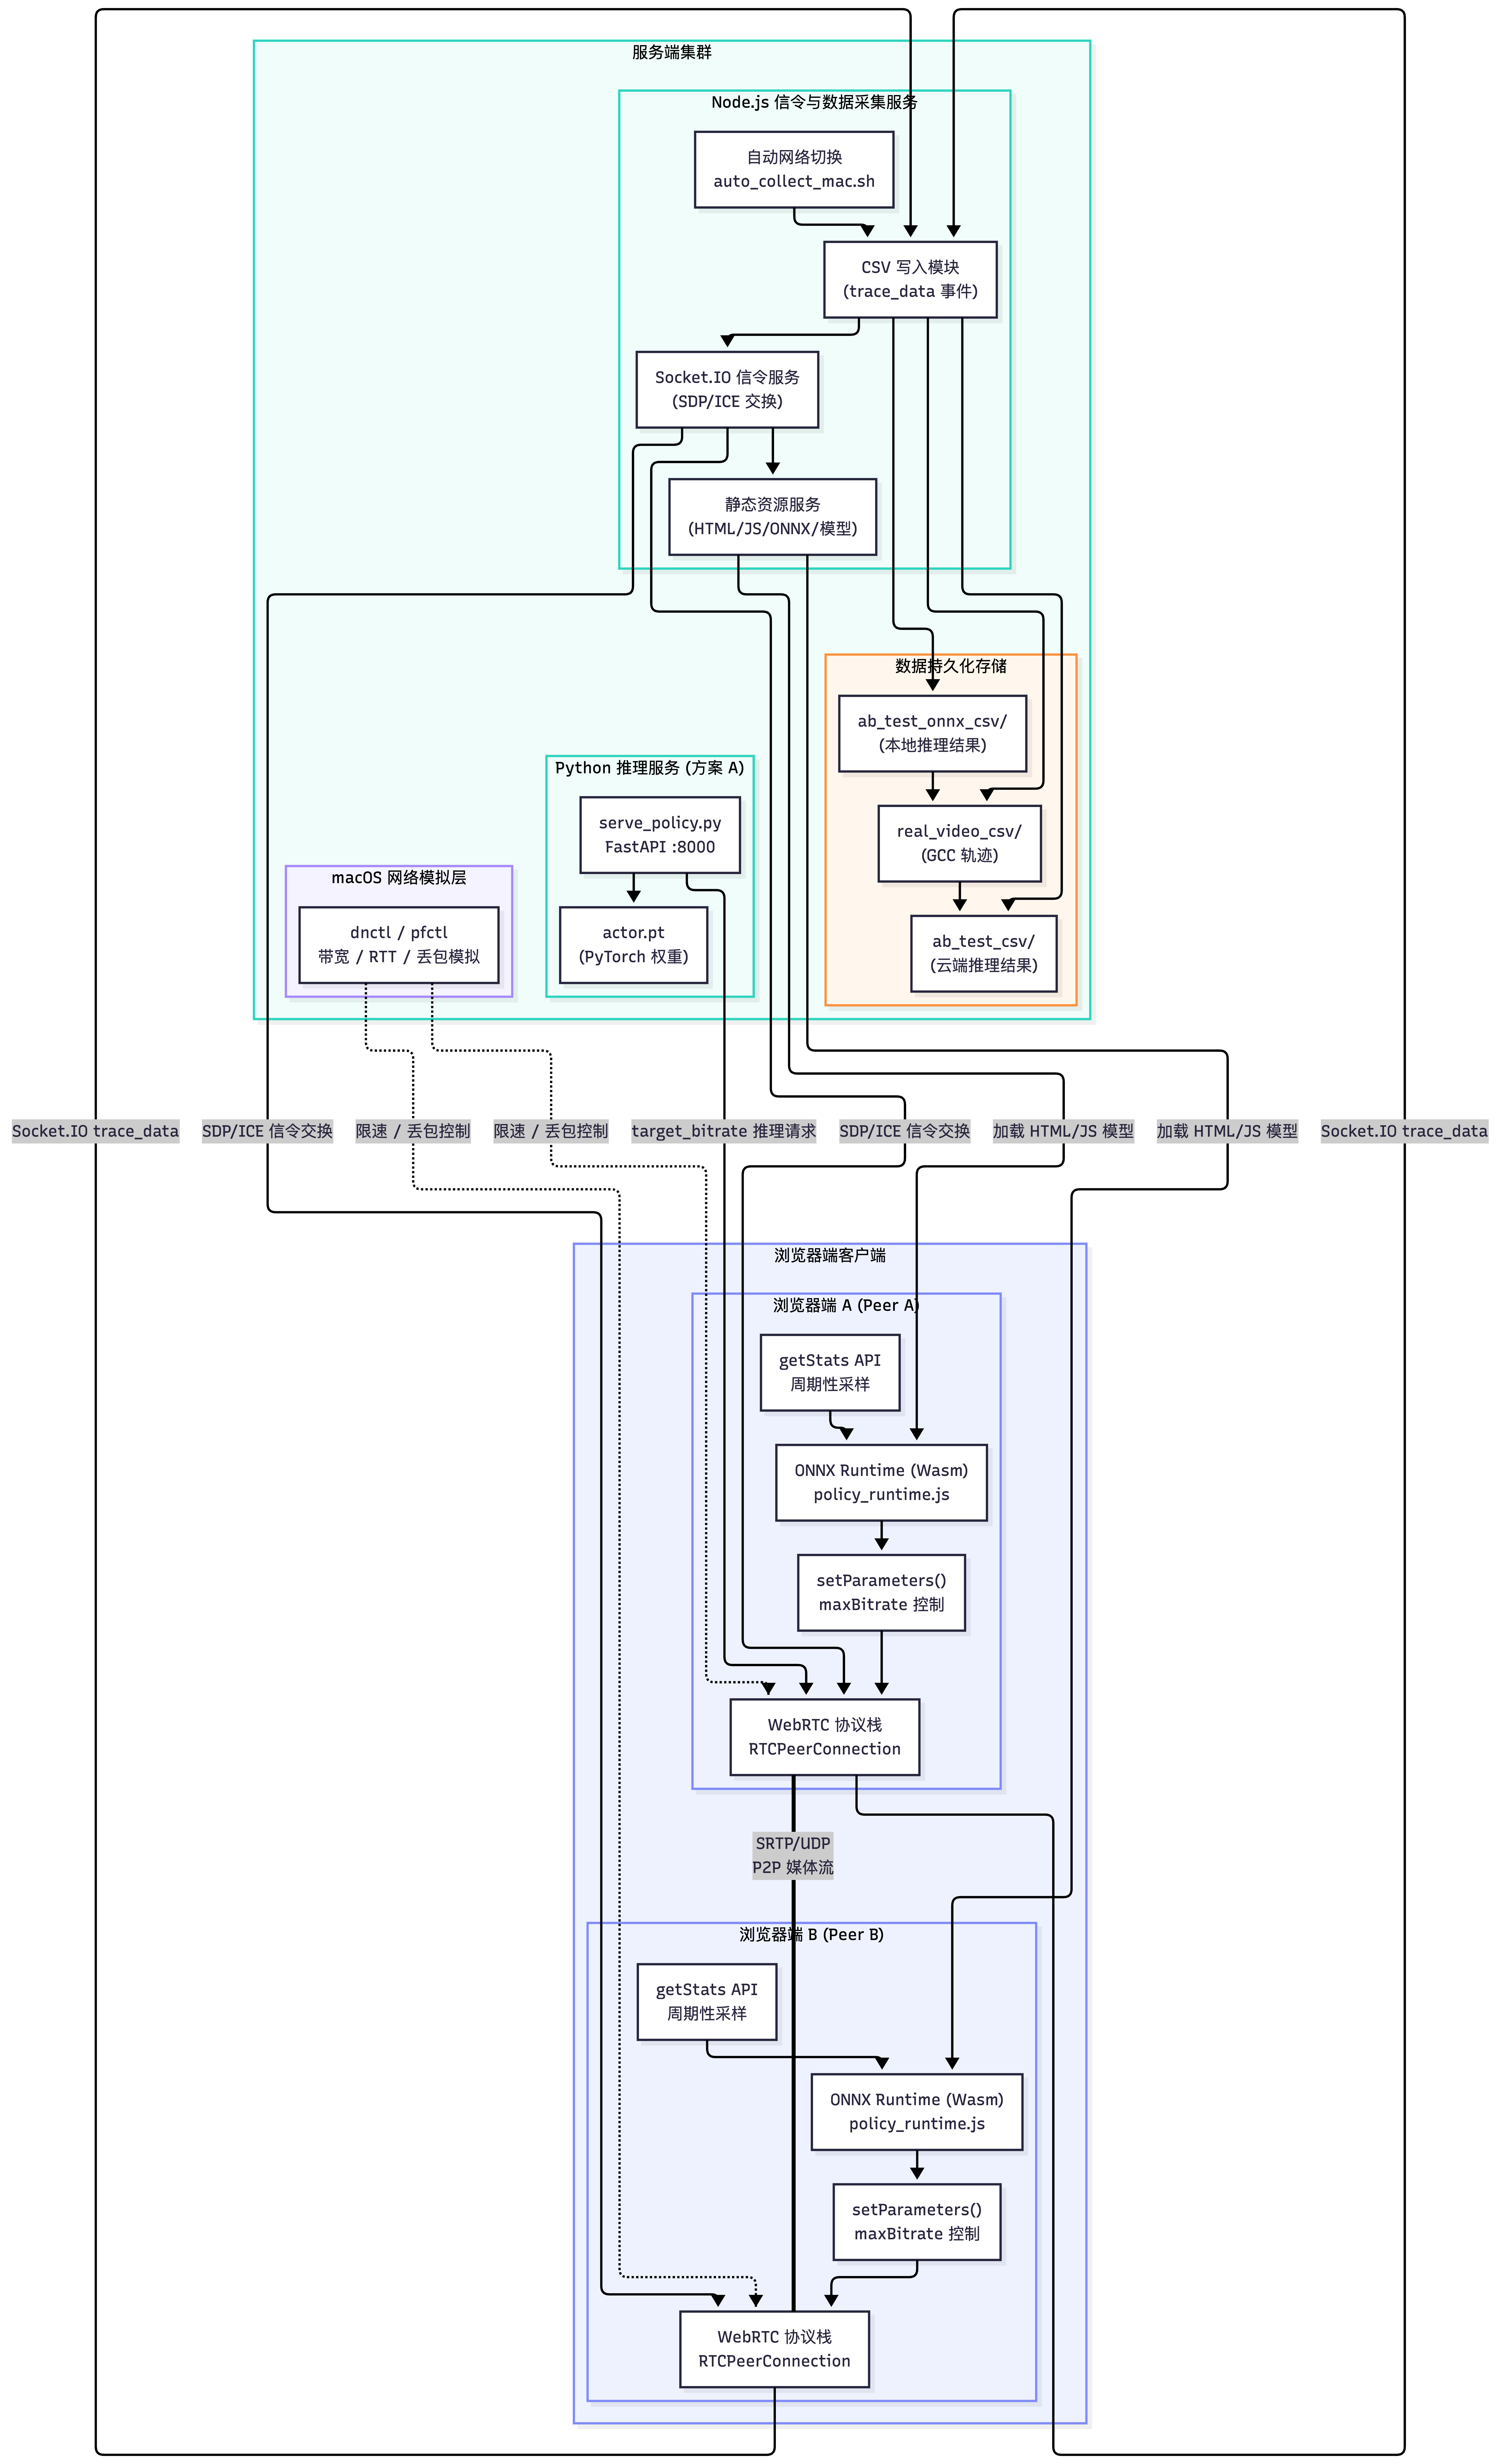
\includegraphics[width=0.8\textwidth]{figures/WebRTC_Peer_Interaction.png}
\caption{WebRTC 采集部署验证平台架构拓扑图}
\label{fig:platform-architecture}
\end{figure}

平台为采集与对照实验分别提供独立的前端入口。图~\ref{fig:trace-collection-frontend} 所示为数据采集界面，提供采集模式选择、当前网络场景指示与本地视频加载入口；操作者通过简单交互即可完成媒体流构建、建立p2p连接、采集网络轨迹数据的全过程。图~\ref{fig:abtest-frontend} 所示为 A/B 测试界面，引入“房间 ID”机制以便两台设备配对，并通过分组下拉框支持对照组（GCC）、实验组（RL 限速）与随机分组三种模式；当会话被分配至实验组时，页面下方的 RL 控制面板自动激活，操作者可在浏览器本地 ONNX 与远端 HTTP 服务两种推理后端之间切换，并实时观察当前作用于 \texttt{maxBitrate} 的限速值，从而直观验证 RL 策略的在线决策行为。

\begin{figure}[htbp]
\centering
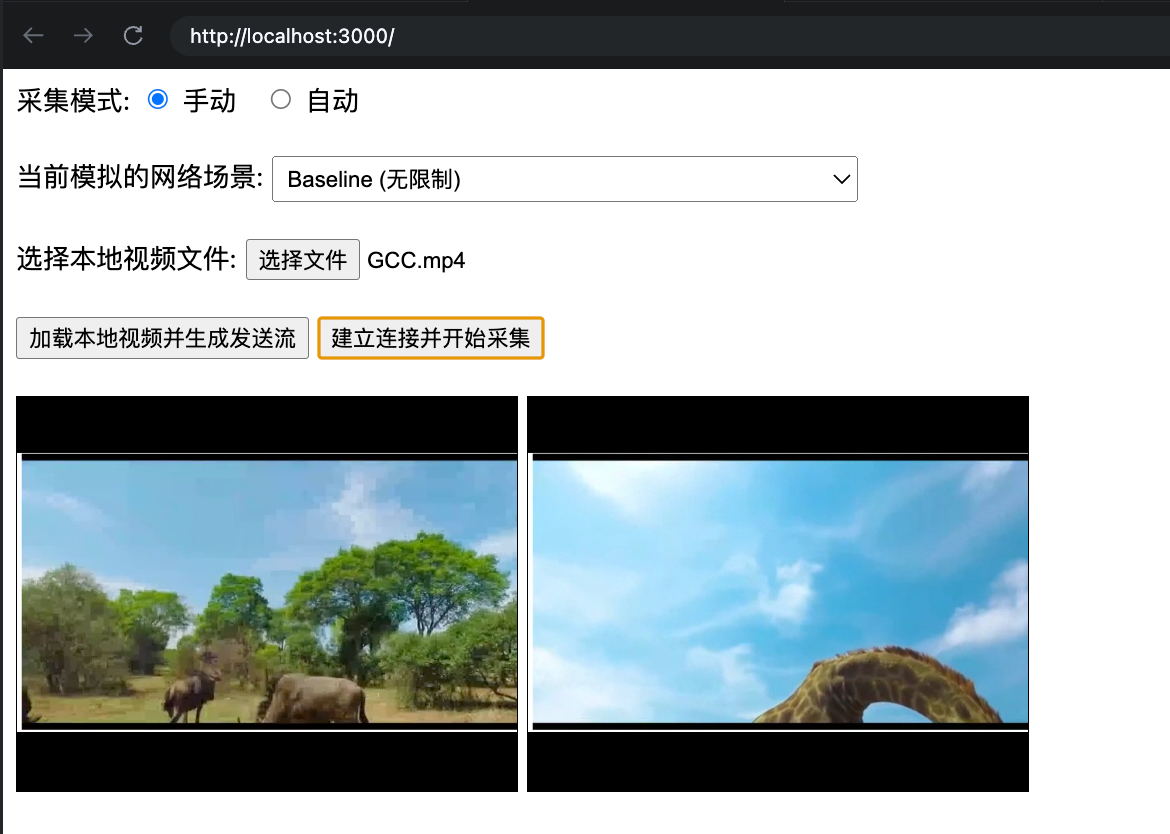
\includegraphics[width=0.85\textwidth]{figures/platform/trace_collection.png}
\caption{数据采集链路前端交互界面}
\label{fig:trace-collection-frontend}
\end{figure}

\begin{figure}[htbp]
\centering
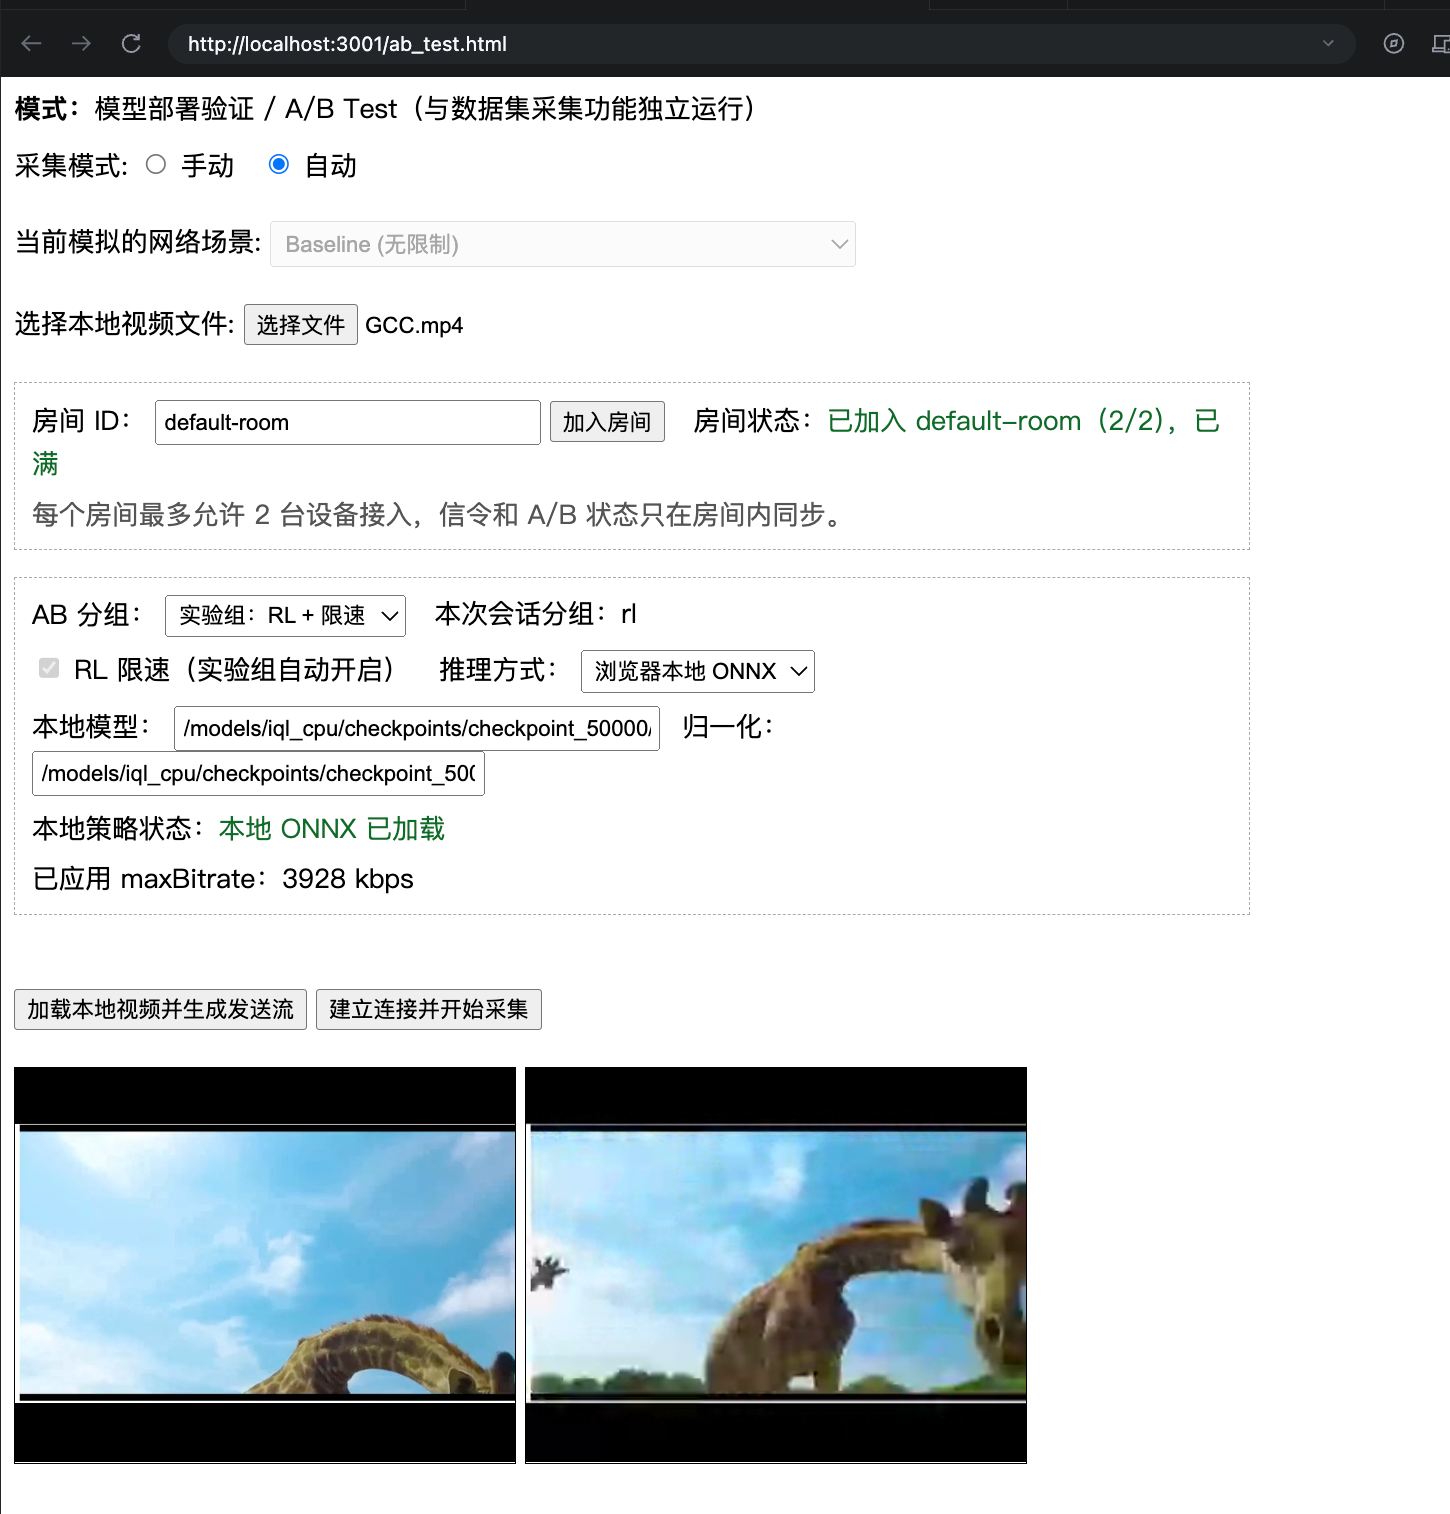
\includegraphics[width=0.85\textwidth]{figures/platform/ab_test.png}
\caption{A/B 测试链路前端交互界面}
\label{fig:abtest-frontend}
\end{figure}

A/B 测试链路在复用基础媒体传输框架的同时，对控制平面的路由逻辑进行了重构。系统在会话建立时执行动态分组仲裁：若被路由至对照组，控制流完全旁路自定义限速逻辑，由浏览器底层 GCC 状态机独立接管码率调度；若被路由至实验组，则在每个采样周期高频触发策略推理流程，由强化学习策略输出码率指令并经 \texttt{setParameters()} 下发。相同物理节点、相同信令体系下的控制流热切换设计，从实验方法学的根源上消除了环境异构性引入的评估偏差，为第~\ref{chap:abtest}~章的对比实验提供了公平基准。

\section{数据采集链路}
\label{sec:collection-pipeline}

数据采集链路的核心目标，是在上述平台框架之下产出具有高真实性与统计代表性的行为数据集。在媒体源层面，发送端利用 HTML5 File API 加载本地测试视频，并通过 \texttt{captureStream()} 接口将其转化为离散的 \texttt{MediaStream} 轨迹，来模拟摄像头采集的数据源。在信令层面，前端通过与 Node.js 服务端的 WebSocket 长连接建立两台设备的建联通道；

媒体通道建立后，前端以 500\,ms 周期触发 \texttt{getStats()} 轮询。从返回值中分别提取下列核心特征量：基于 \texttt{bytesSent}/\texttt{bytesReceived} 差分计算得到的发送与接收吞吐量，源自 \texttt{candidate-pair} 的物理往返时延 RTT，源自 \texttt{inbound-rtp} 的接收端抖动 Jitter，基于序列号连续性统计的丢包率，以及由原生 GCC 算法输出的可用带宽估计 \texttt{availableOutgoingBitrate}。每个采样点连同时间戳与客户端标识被序列化为结构化记录，经 WebSocket 实时回传至服务端，并以\texttt{webrtc\_network\_traces\_<scenario>\_<traceStartTs>.csv} 的命名规范追加落盘。其中 \texttt{<scenario>} 标签由网络控制脚本动态注入，\texttt{<traceStartTs>} 标记一次连续会话的起始时刻。

\section{专家策略数据集的收集和预处理}
\label{sec:expert-dataset}

离线强化学习的训练数据必须由一个安全、稳定且工程上可用的行为策略生成。本文选择浏览器默认搭载的 GCC 算法作为专家策略 $\pi_E$，理由有二：其一，GCC 作为业界主流的启发式拥塞控制算法已在大规模生产系统中长期验证，能够在多数网络条件下提供稳定的基线体验。其二，由于浏览器中默认搭载的拥塞控制算法就是 GCC 算法，因此天然适配本文基于浏览器的数据采集平台，

为获取覆盖多种典型网络环境下的行为数据，自动采集模式下，服务端在每次会话建立时，会调用 macOS 的 \texttt{dnctl}/\texttt{pfctl}（dummynet）对宿主机所有出入方向流量施加整形规则，并以五分钟为周期在九类网络环境之间轮询。每次场景切换时脚本生成新的 \texttt{traceStartTs} 并通过 HTTP 接口广播至前端，前端随即开启新的轨迹片段，从而保证每个片段内部的网络参数保持平稳。九类场景的具体参数化设计见表~\ref{tab:network-profiles-9}。需要强调的是，该参数表并非用于“仿真网络”，而是为了在真实 WebRTC 协议栈之上构造一组可控、可复现且覆盖带宽、时延、丢包与非平稳波动等关键劣化维度的物理信道条件，进而获得具有代表性的 GCC 行为数据集。同时，\texttt{scenario} 标签也作为后续 A/B 测试阶段的统一实验条件标识，实现了采集分桶与评测分桶的严格一致。

\begin{table}[htbp]
\centering
\small
\begin{tabular}{|l|c|c|c|p{5.8cm}|}
\hline
场景标签 & 带宽 & 延迟 & 丢包率 & 设计目的 \\
\hline
\texttt{baseline} & 1000 Mbit/s & 0 ms & 0\% & 理想链路基线，用于验证采集链路完备性与高质量网络下的上界表现 \\
\hline
\texttt{3g} & 555 Kbit/s & 100 ms & 0\% & 低带宽 + 中等时延的蜂窝弱网，考察吞吐受限下的保守性 \\
\hline
\texttt{lte} & 30 Mbit/s & 58 ms & 0\% & 高容量蜂窝网络，考察延迟约束下的码率选择 \\
\hline
\texttt{dsl} & 1128 Kbit/s & 5 ms & 0\% & 低带宽且低 RTT 的典型宽带接入场景 \\
\hline
\texttt{low\_bw} & 500 Kbit/s & 0 ms & 0\% & 极低稳定带宽上限，考察持续瓶颈下的目标码率收敛 \\
\hline
\texttt{high\_loss} & 10 Mbit/s & 0 ms & 5\% & 中等带宽下的持续随机丢包，考察非拥塞性丢包鲁棒性 \\
\hline
\texttt{high\_delay} & 5 Mbit/s & 150 ms & 0\% & 中等带宽下的高 RTT，考察对延迟惩罚的响应 \\
\hline
\texttt{fluctuating} & 多阶段时变 & 多阶段时变 & 多阶段时变 & 单窗口内按时间表阶梯切换，模拟非平稳网络与突发事件 \\
\hline
\texttt{very\_bad} & 1 Mbit/s & 500 ms & 10\% & 极端弱网，用于压力测试与策略失效边界分析 \\
\hline
\end{tabular}
\caption{自动采集模式下的九类网络环境配置}
\label{tab:network-profiles-9}
\end{table}

真实 WebRTC 采集数据与仿真器产出的理想化轨迹存在本质差异。\texttt{getStats()} 接口在实际运行中通常会暴露三类典型缺陷：第一，\textbf{周期性零点异常}，即 WebRTC 内部统计模块在尚未完成一轮完整测量的时间窗口内，对 RTT 与带宽估计等指标暂时返回零值或空值，但同时段的吞吐量字段仍维持正常，相邻采样点亦为合理非零值；第二，\textbf{短暂缺失段}，由于浏览器主线程阻塞、垃圾回收或标签页切换等原因导致的连续 1–3 个采样周期字段缺失，此类缺失并不反映真实链路中断；第三，\textbf{长期断裂段}，当网络场景切换发生时，轨迹中会出现长达数十秒的连续缺失区间，此区间内的网络状态不可推测，若强行插值将引入严重伪轨迹。三类缺陷如未在训练集构建之前妥善处理，将污染状态分布并导致价值函数在虚假区域过拟合，最终损害策略的部署可靠性。

针对上述缺陷，本文设计了“异常零点标记—短缺失插值—长断裂切段”三级清洗流程。在异常零点识别阶段，仅当某行 RTT 或 GCC 估计带宽为零或负值，且同时满足“流量活跃性条件”（同行其余流量字段至少有一项为正）与“相邻非零条件”（前后行为正值）时，将其判定为采样伪影并标记为 NaN；该判别准则的核心思想在于，孤立零值若被两侧合理样本与持续吞吐所包围，更可能源于 \texttt{getStats()} 在当前周期内未完成 RTCP 往返测量，而非物理意义上的瞬时跌零。在短缺失修复阶段，对长度不超过三个采样周期的连续 NaN 区间执行分段线性插值；该阈值的选取依据是，三秒内的 RTT 与吞吐量变化在典型 WiFi 与蜂窝网络中可被线性趋势合理近似，超过该阈值后的区间则可能跨越场景切换或链路断开，线性外推不再具有物理可信度。在长断裂切段阶段，依据连续完整性标记将原始轨迹拆分为若干长度不等的有效段，并赋予独立的 \texttt{segment\_id}；该编号在后续滑动窗口构建时用作硬隔离边界，保证窗口永不跨越数据断裂区间。

为保证清洗策略对真实数据的有效性可被人工审查，本文对九类网络场景共 152 段会话的原始 CSV 文件逐一生成“原始轨迹 vs 修复后轨迹”对比图，每张对比图涵盖 RTT、Jitter、丢包率、接收吞吐量与 GCC 估计带宽五项关键指标。代表性场景的对比结果展示于图~\ref{fig:traces-row1}–\ref{fig:traces-row3}。从可视化结果可以观察到三方面事实：其一，原始轨迹呈现出与 dnctl 限速参数高度吻合的物理动态，例如 3G 场景下吞吐量受 555\,Kbps 上限明显截断而 RTT 因排队效应升高至数百毫秒量级，fluctuating 场景下吞吐量呈现出与脚本预设时间表一致的阶梯式跃变；其二，原始轨迹中确实存在 ICE 建立期的零点序列、浏览器进程暂停产生的时间断裂以及个别物理上不合理的瞬时突变；其三，清洗流程有效消除了上述伪影而未破坏真实拥塞信号——短期零点被插值平滑填充，长断裂被切分为独立片段以避免虚假时序依赖，而正常的带宽下降与 RTT 上升均完整保留。该可视化审查为后续训练数据的物理可信度提供了人工校验关卡。

\begin{figure}[htbp]
\centering
\begin{minipage}{0.32\textwidth}
\centering
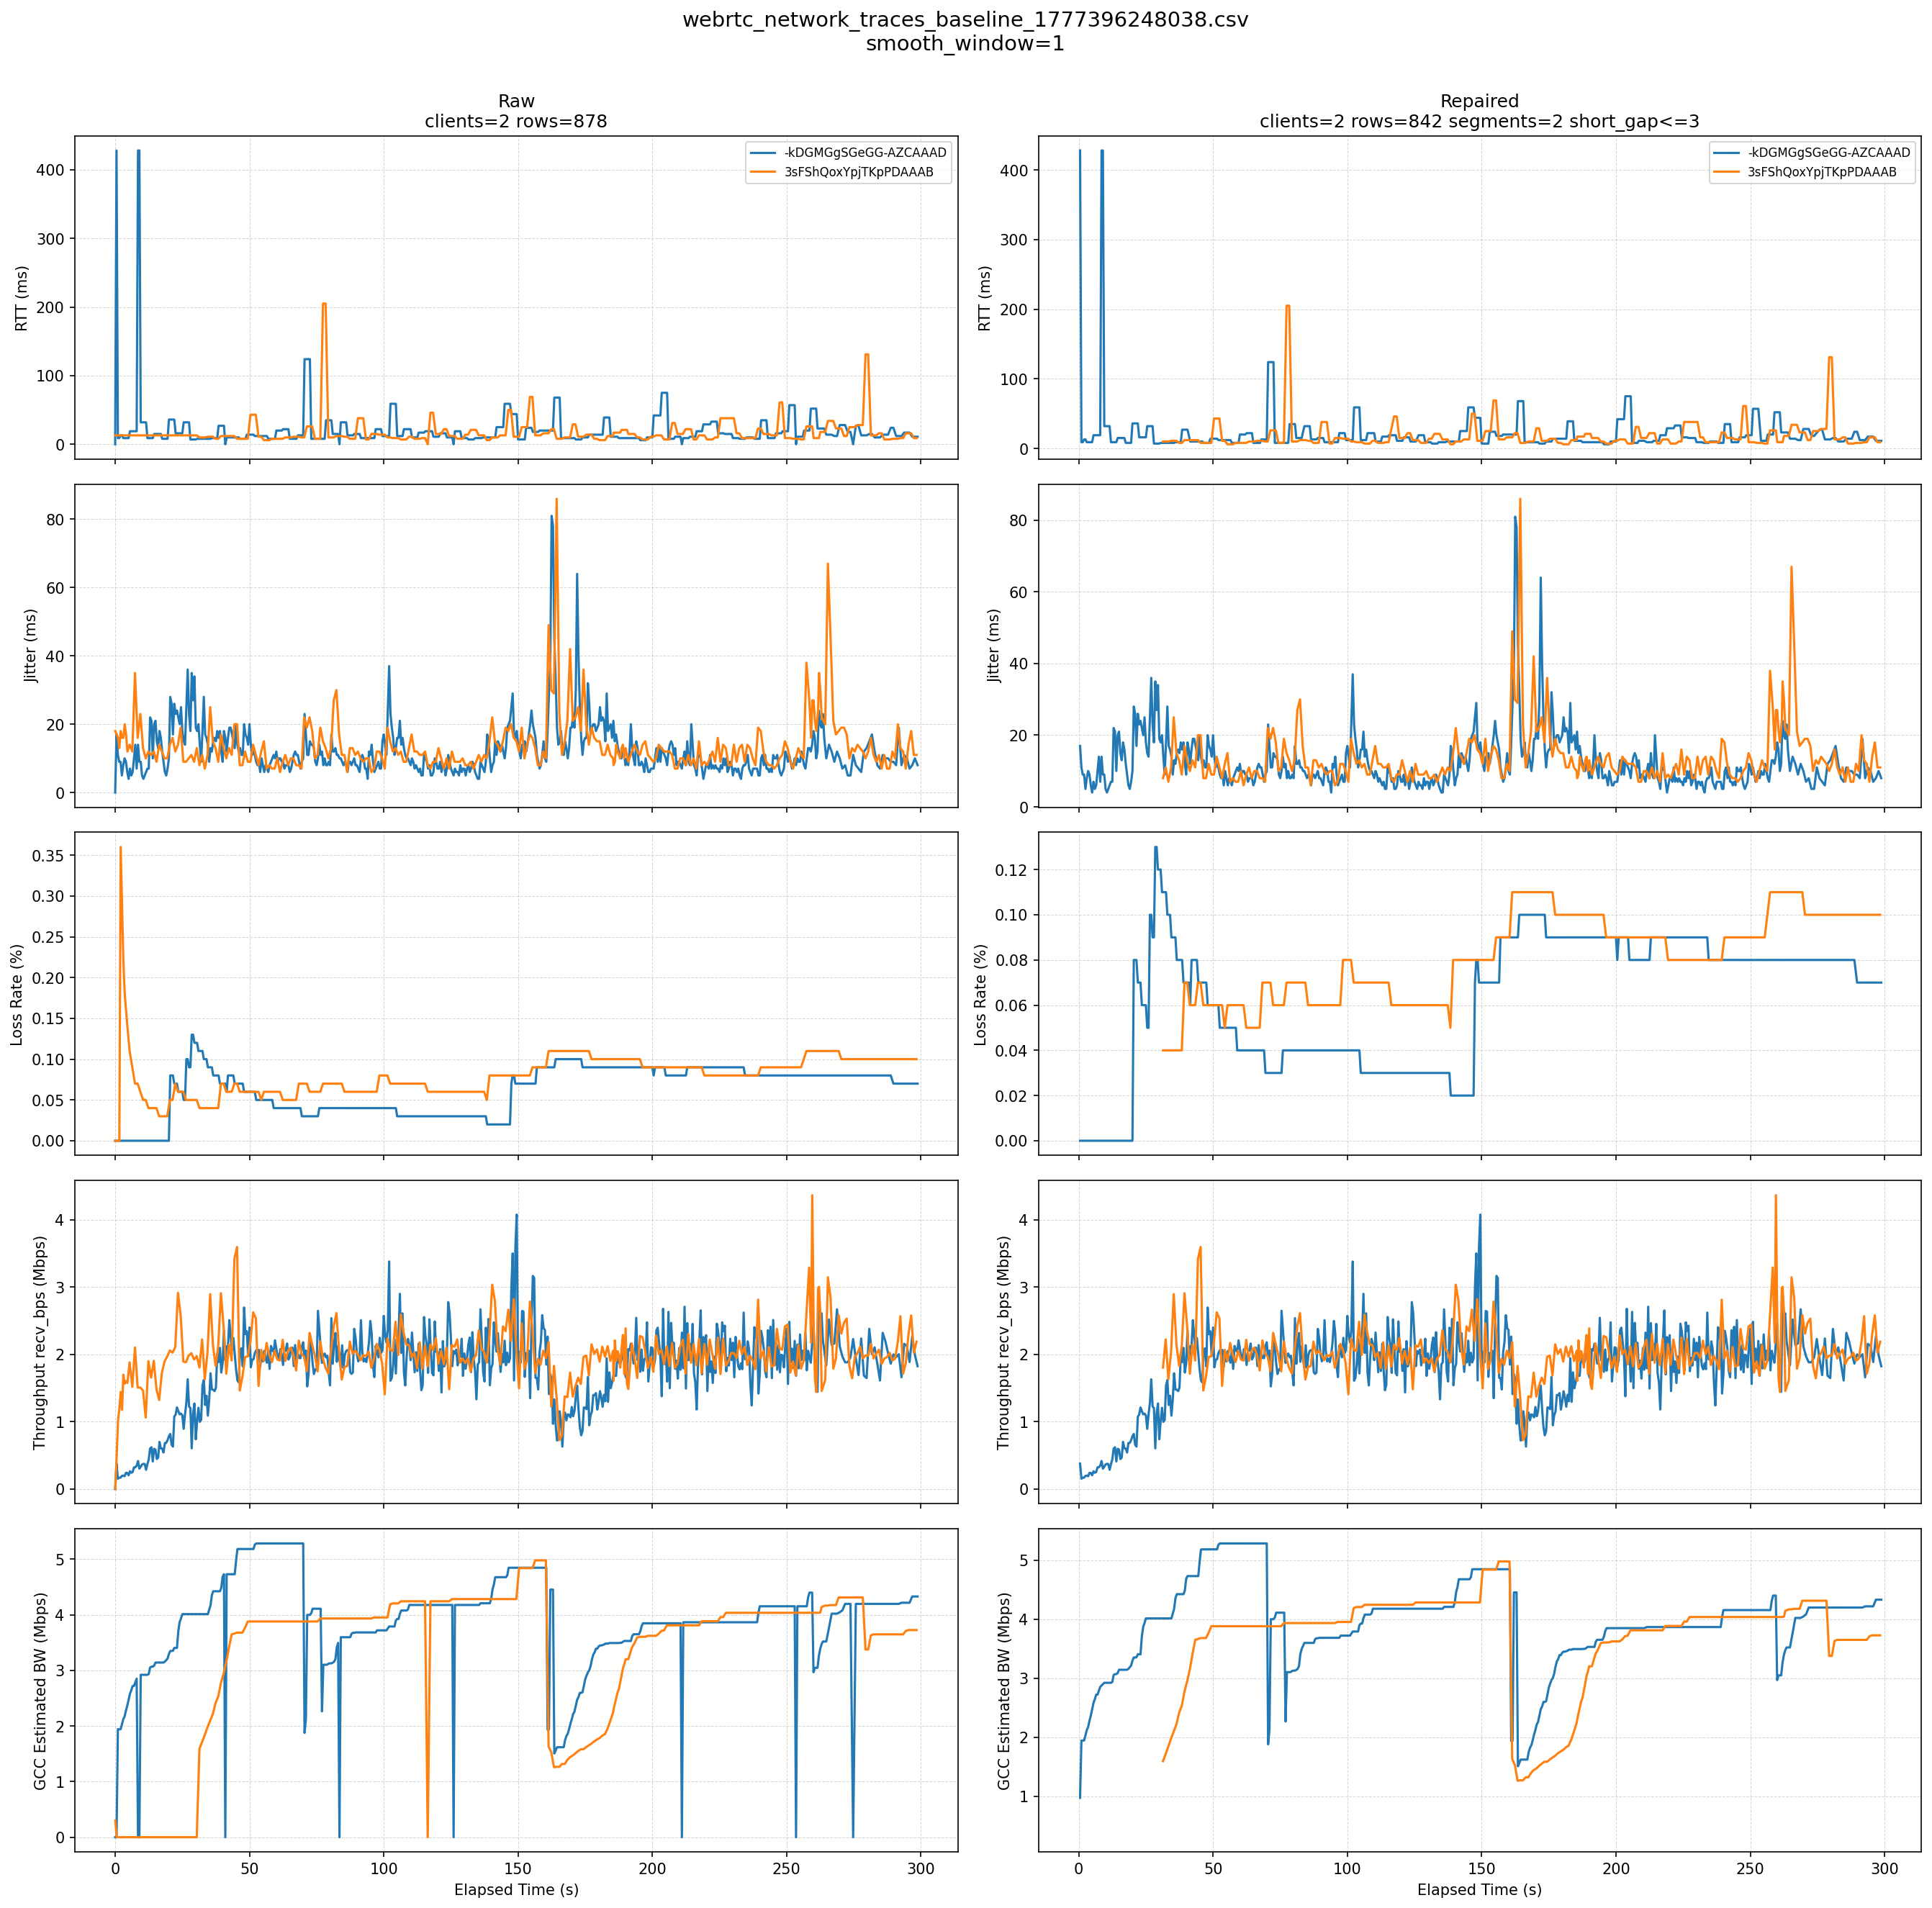
\includegraphics[width=\textwidth]{figures/traces/baseline_trace_8038.png}
\subcaption{baseline}
\end{minipage}\hfill
\begin{minipage}{0.32\textwidth}
\centering
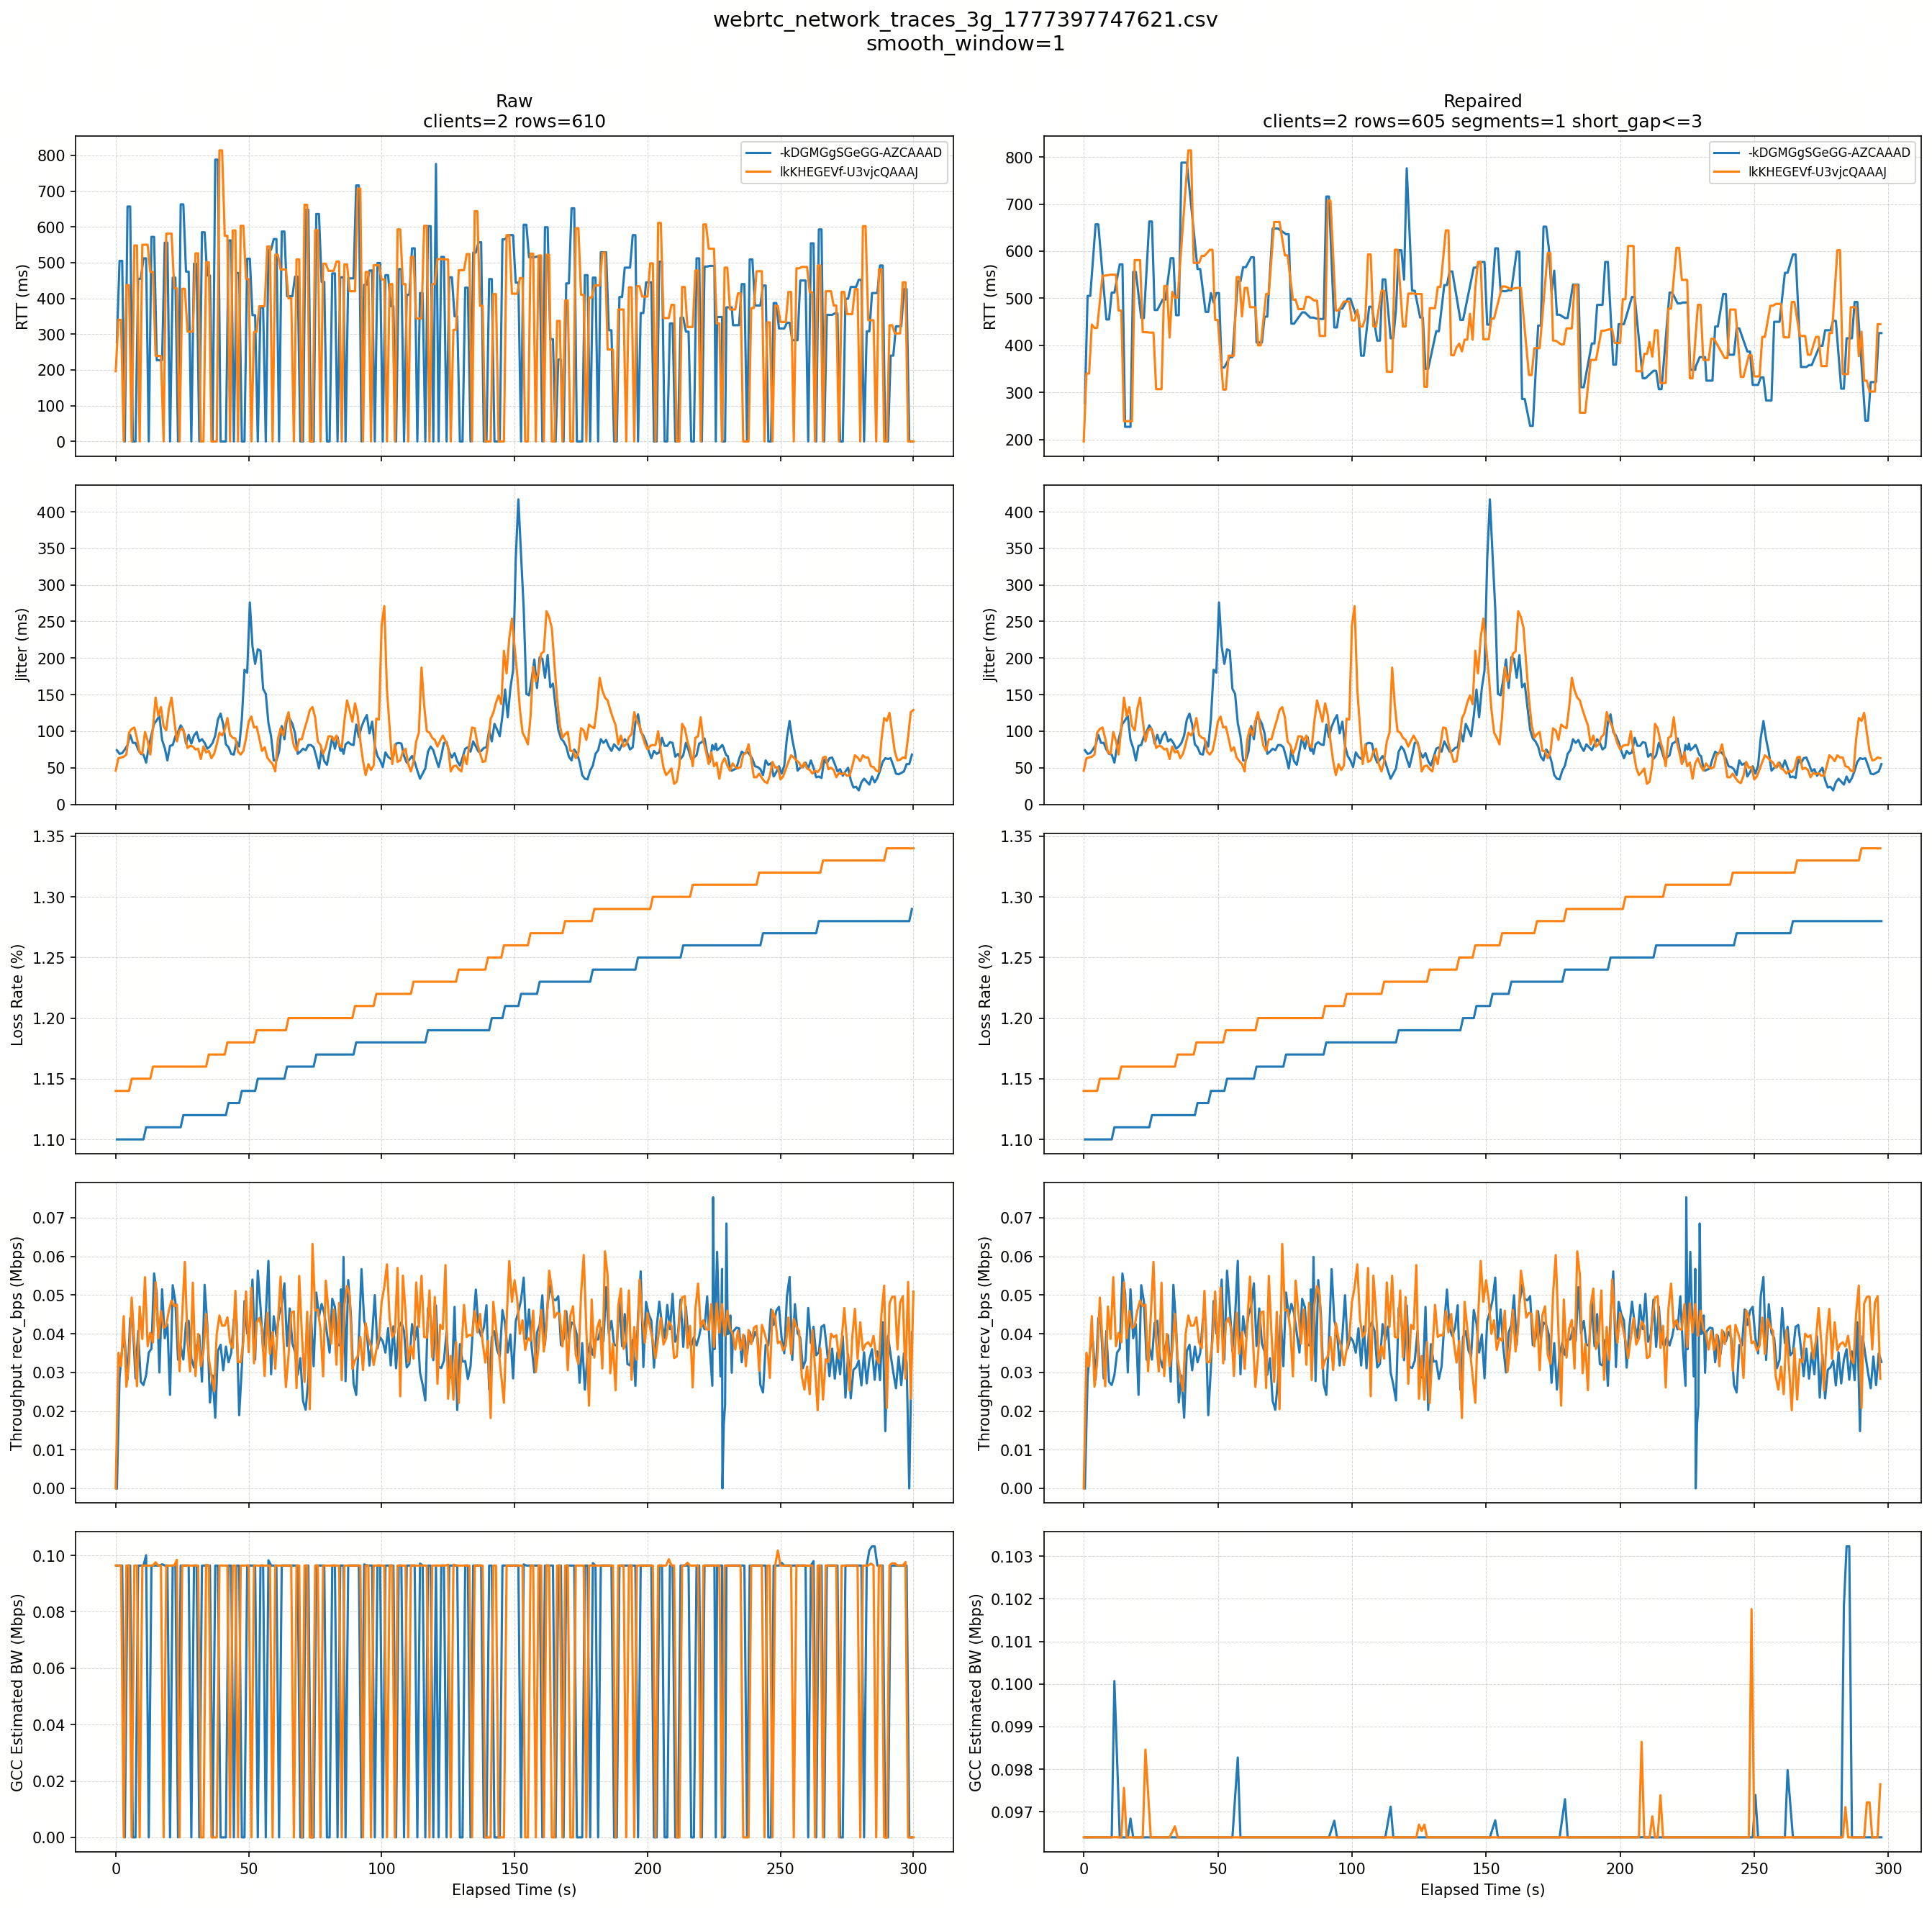
\includegraphics[width=\textwidth]{figures/traces/3g_trace_7621.png}
\subcaption{3g}
\end{minipage}\hfill
\begin{minipage}{0.32\textwidth}
\centering
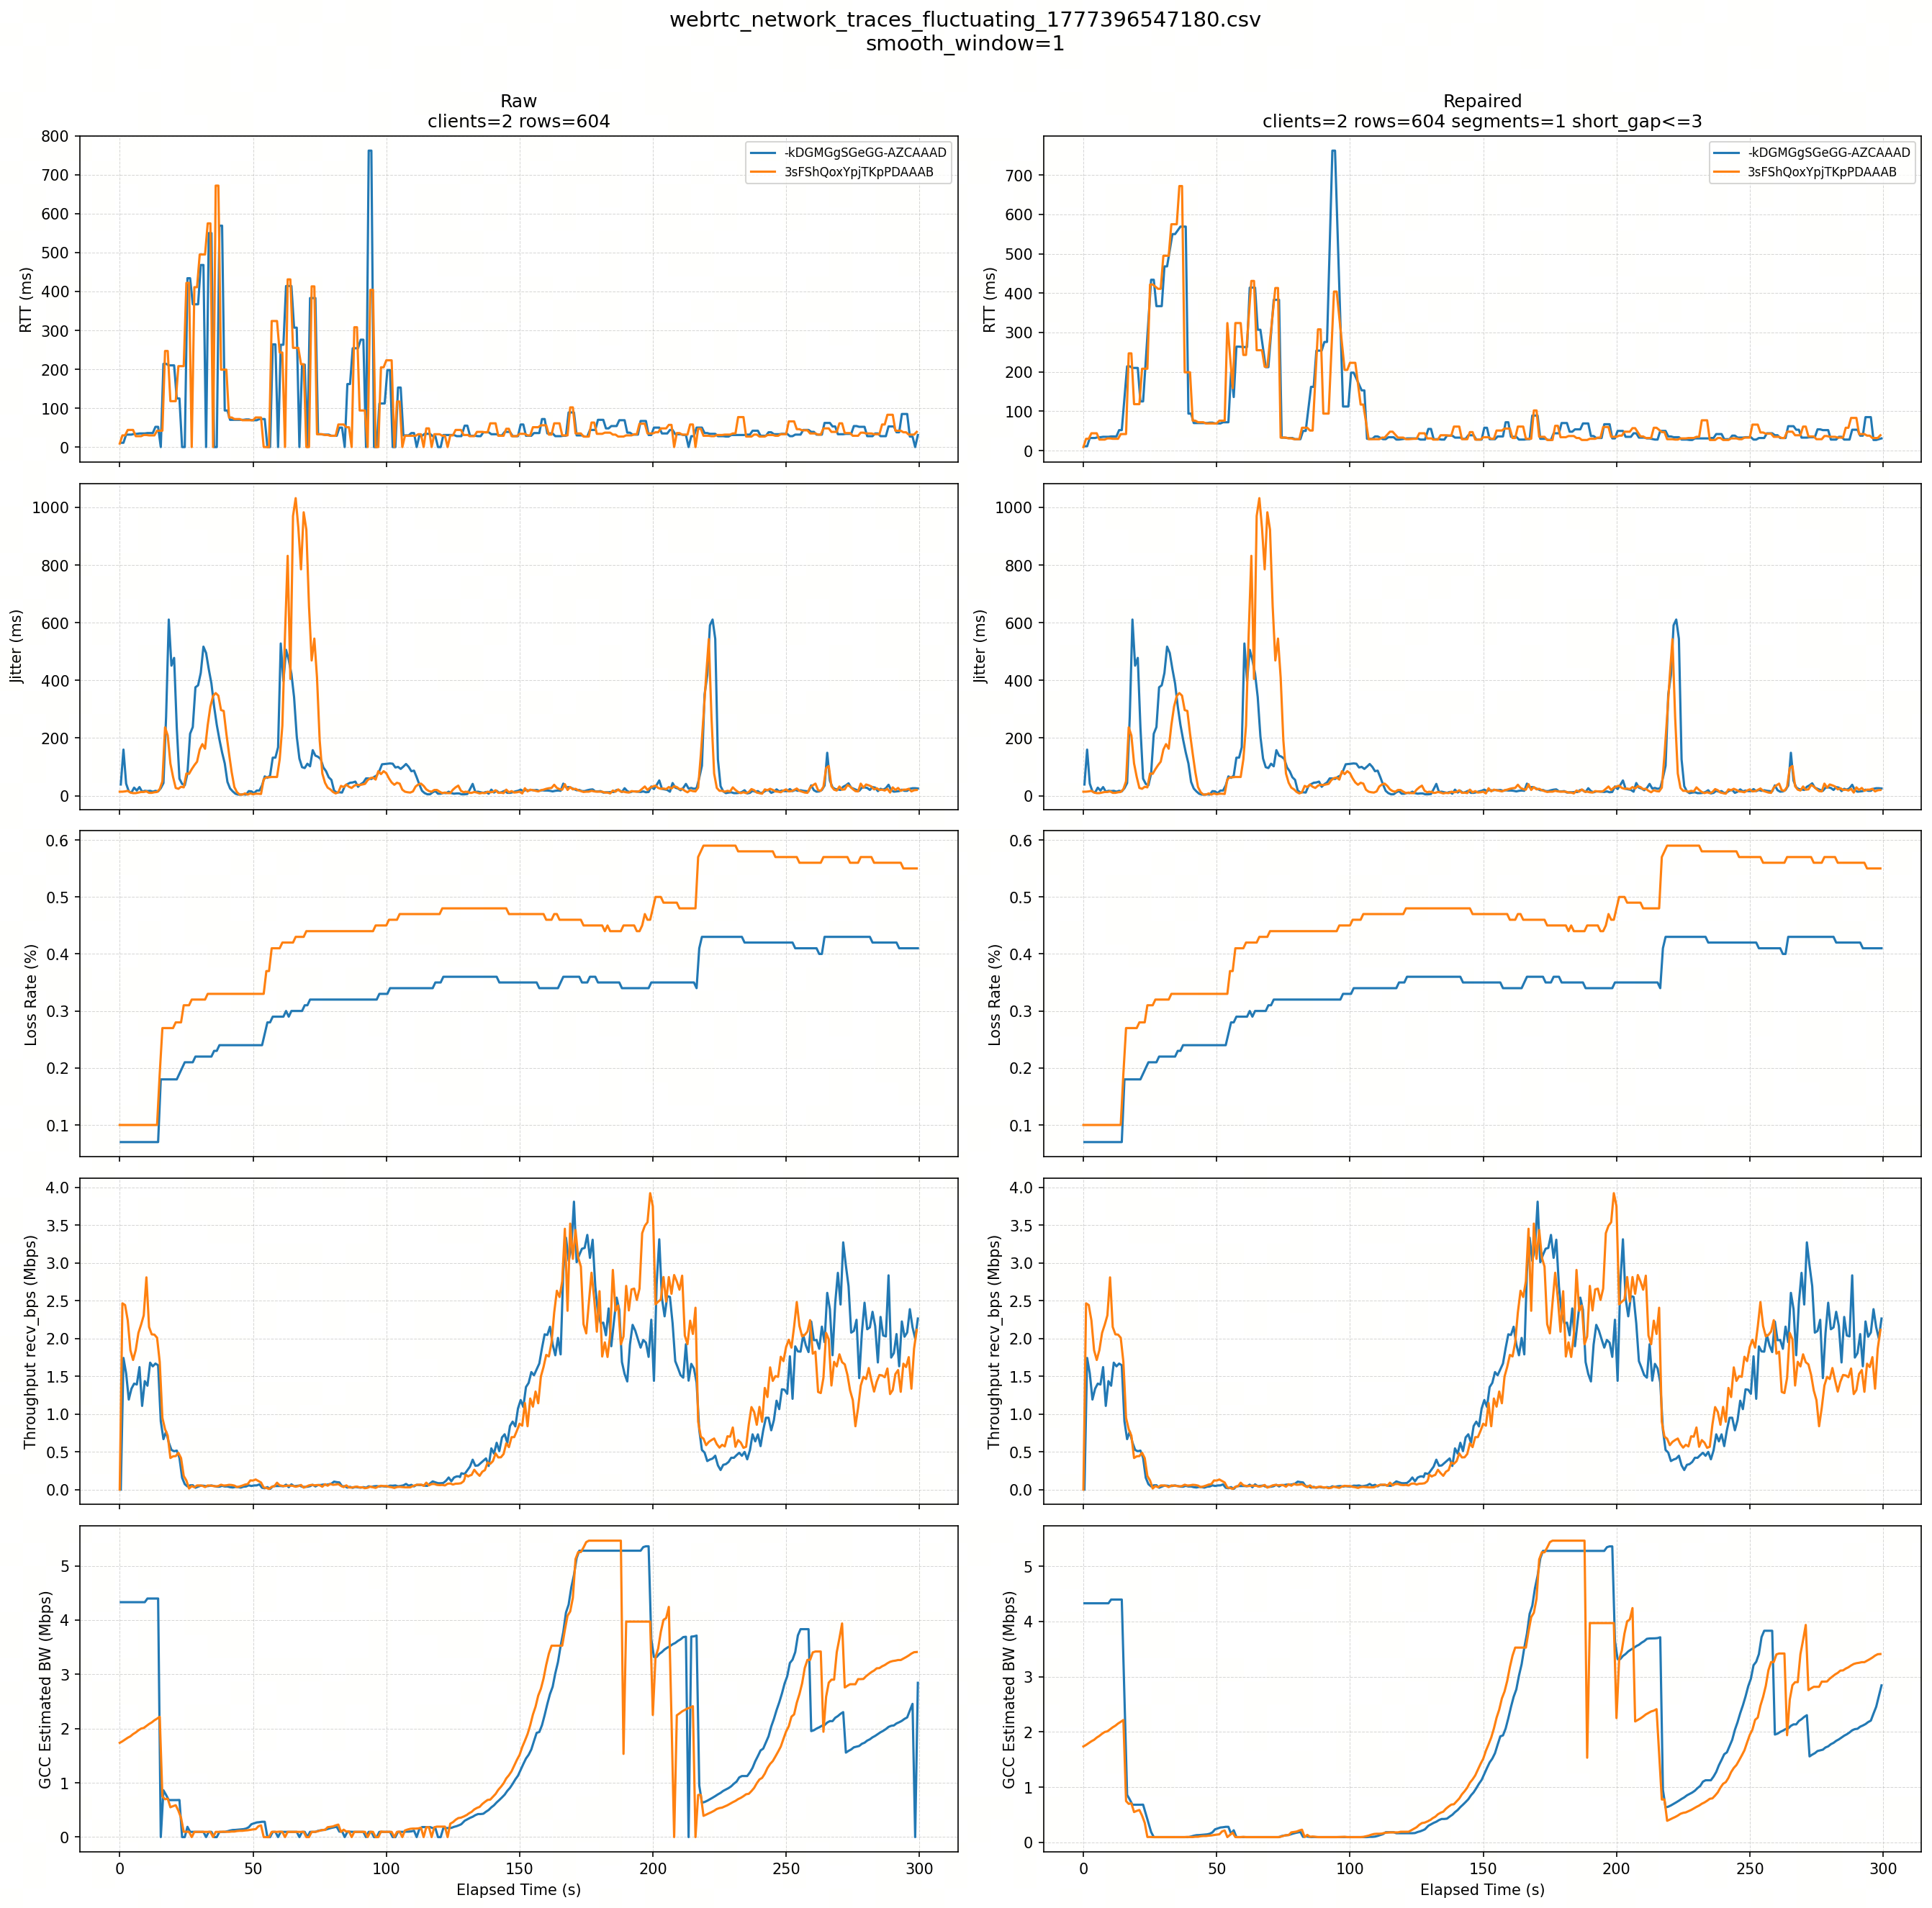
\includegraphics[width=\textwidth]{figures/traces/fluctuating_trace_7180.png}
\subcaption{fluctuating}
\end{minipage}
\caption{典型场景下的原始/修复轨迹对比（一）}
\label{fig:traces-row1}
\end{figure}

\begin{figure}[htbp]
\centering
\begin{minipage}{0.32\textwidth}
\centering
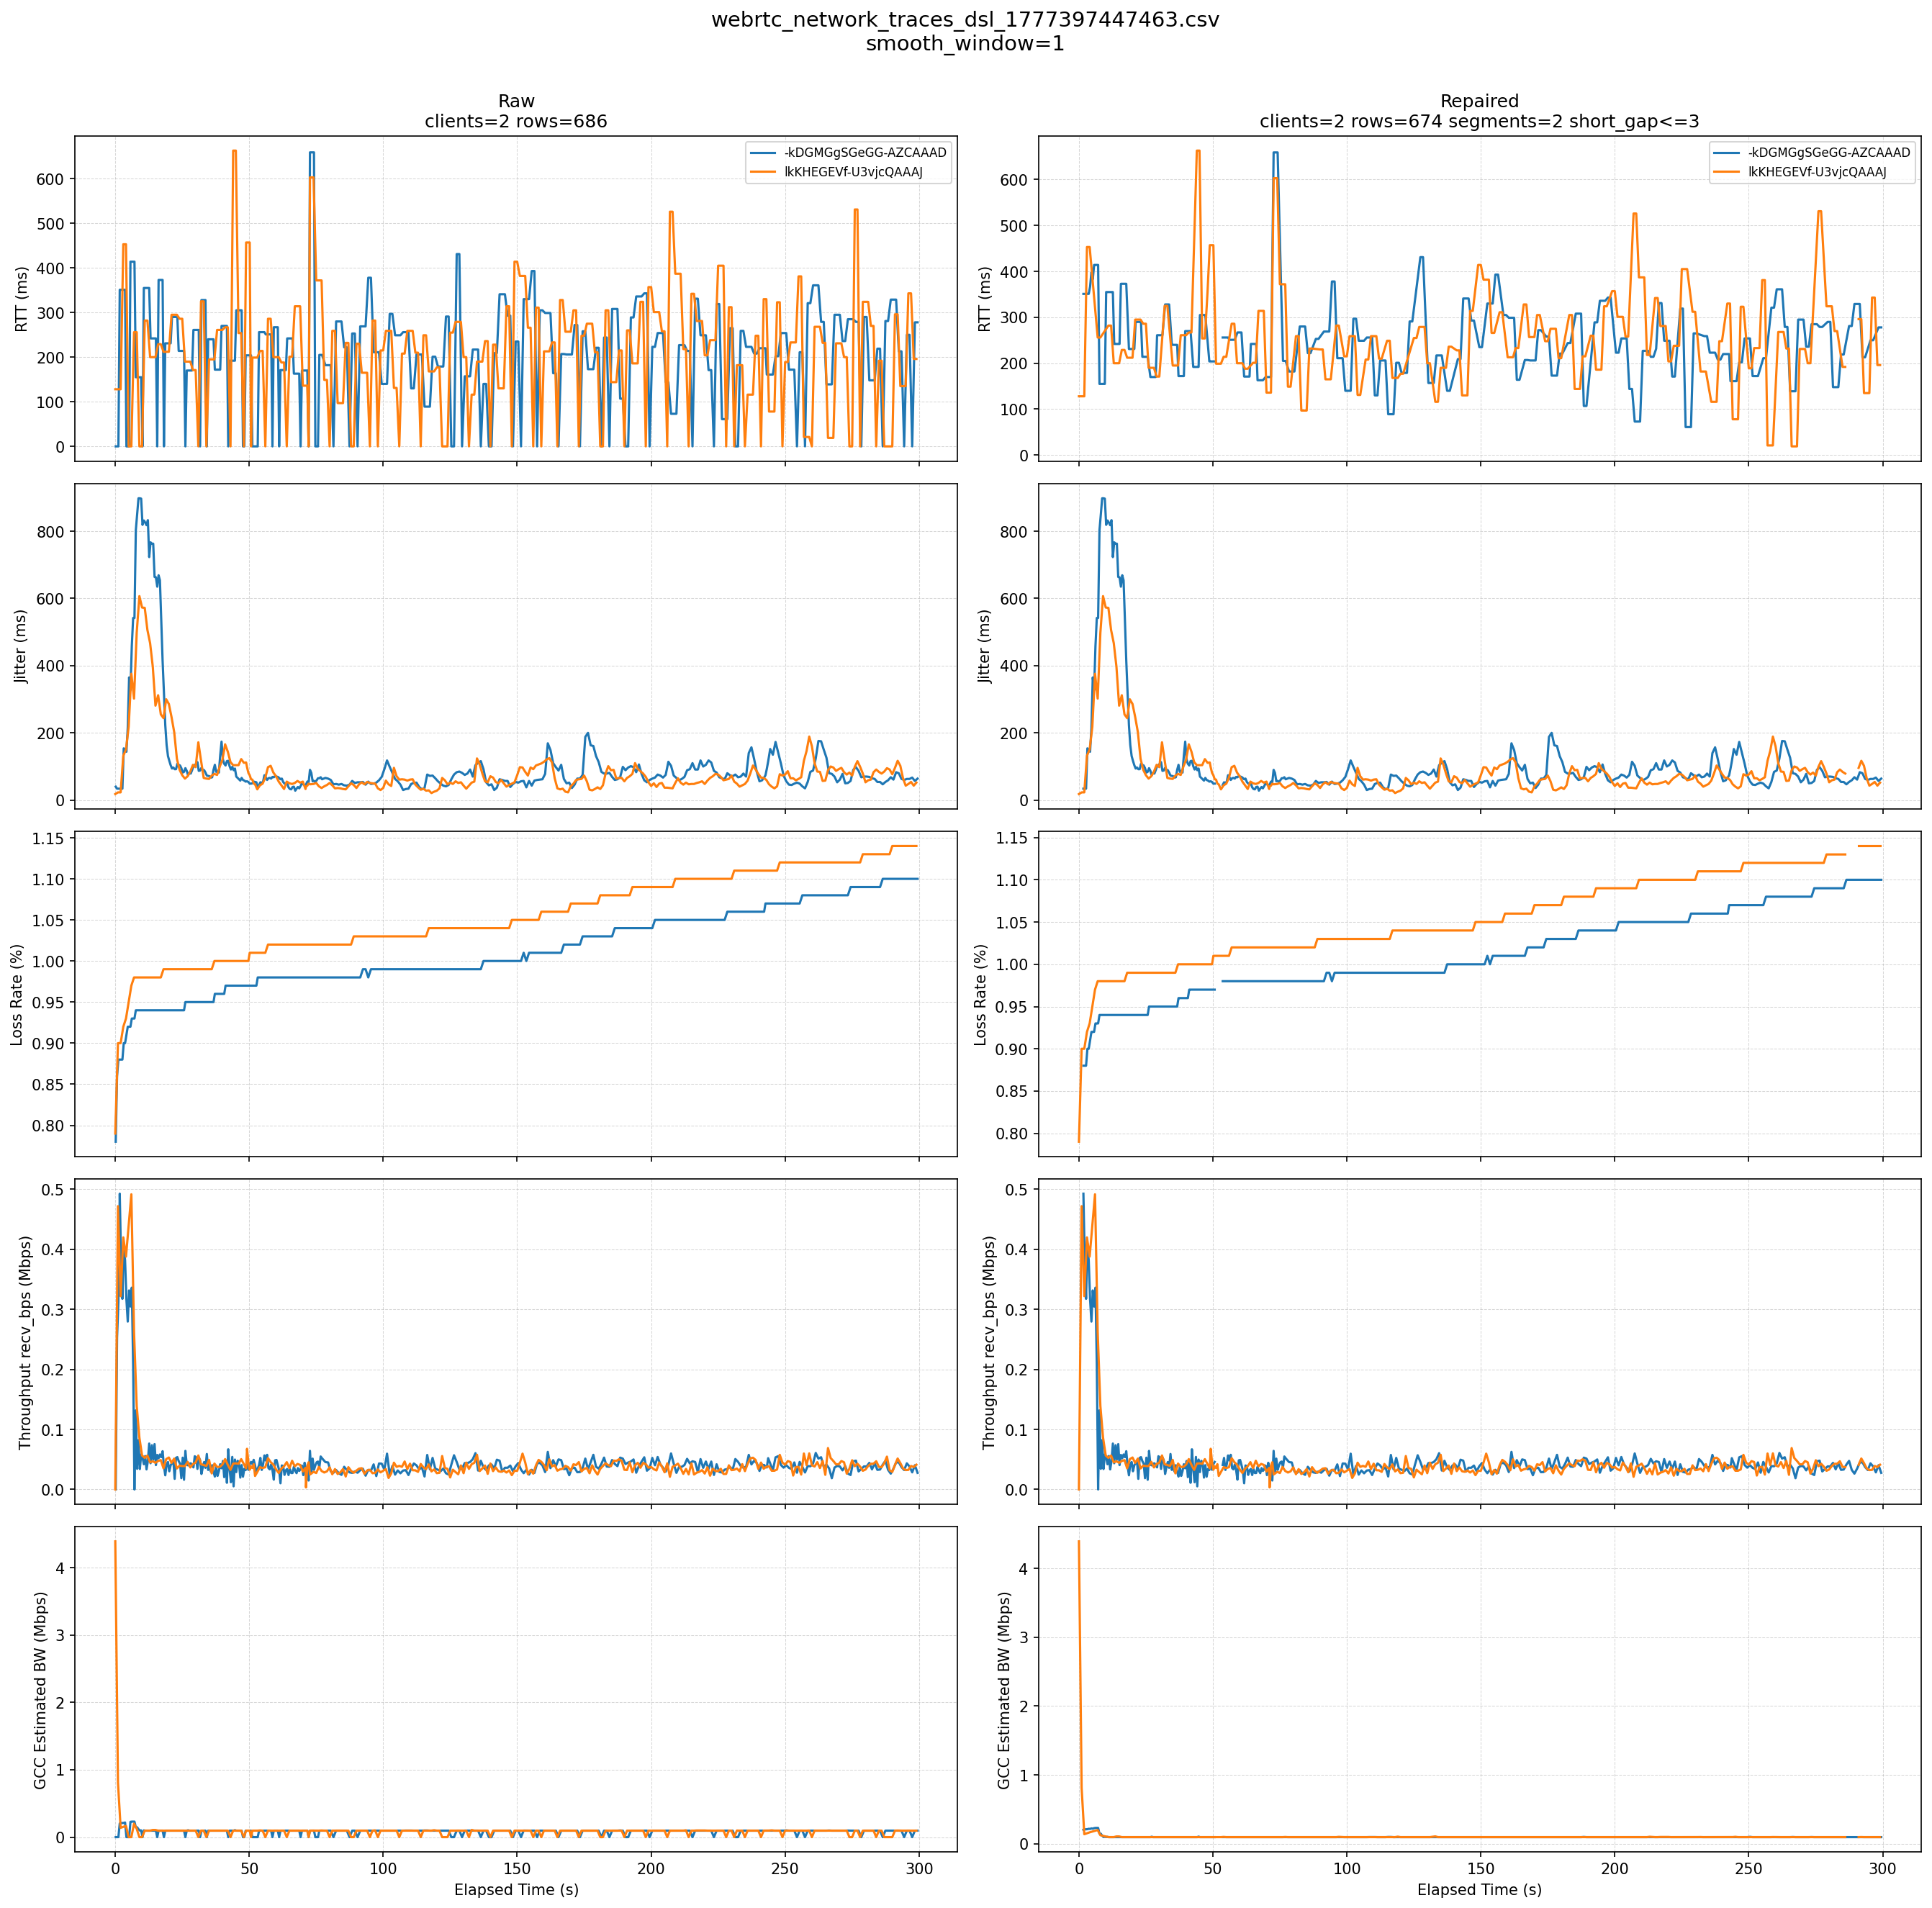
\includegraphics[width=\textwidth]{figures/traces/dsl_trace_7463.png}
\subcaption{dsl}
\end{minipage}\hfill
\begin{minipage}{0.32\textwidth}
\centering
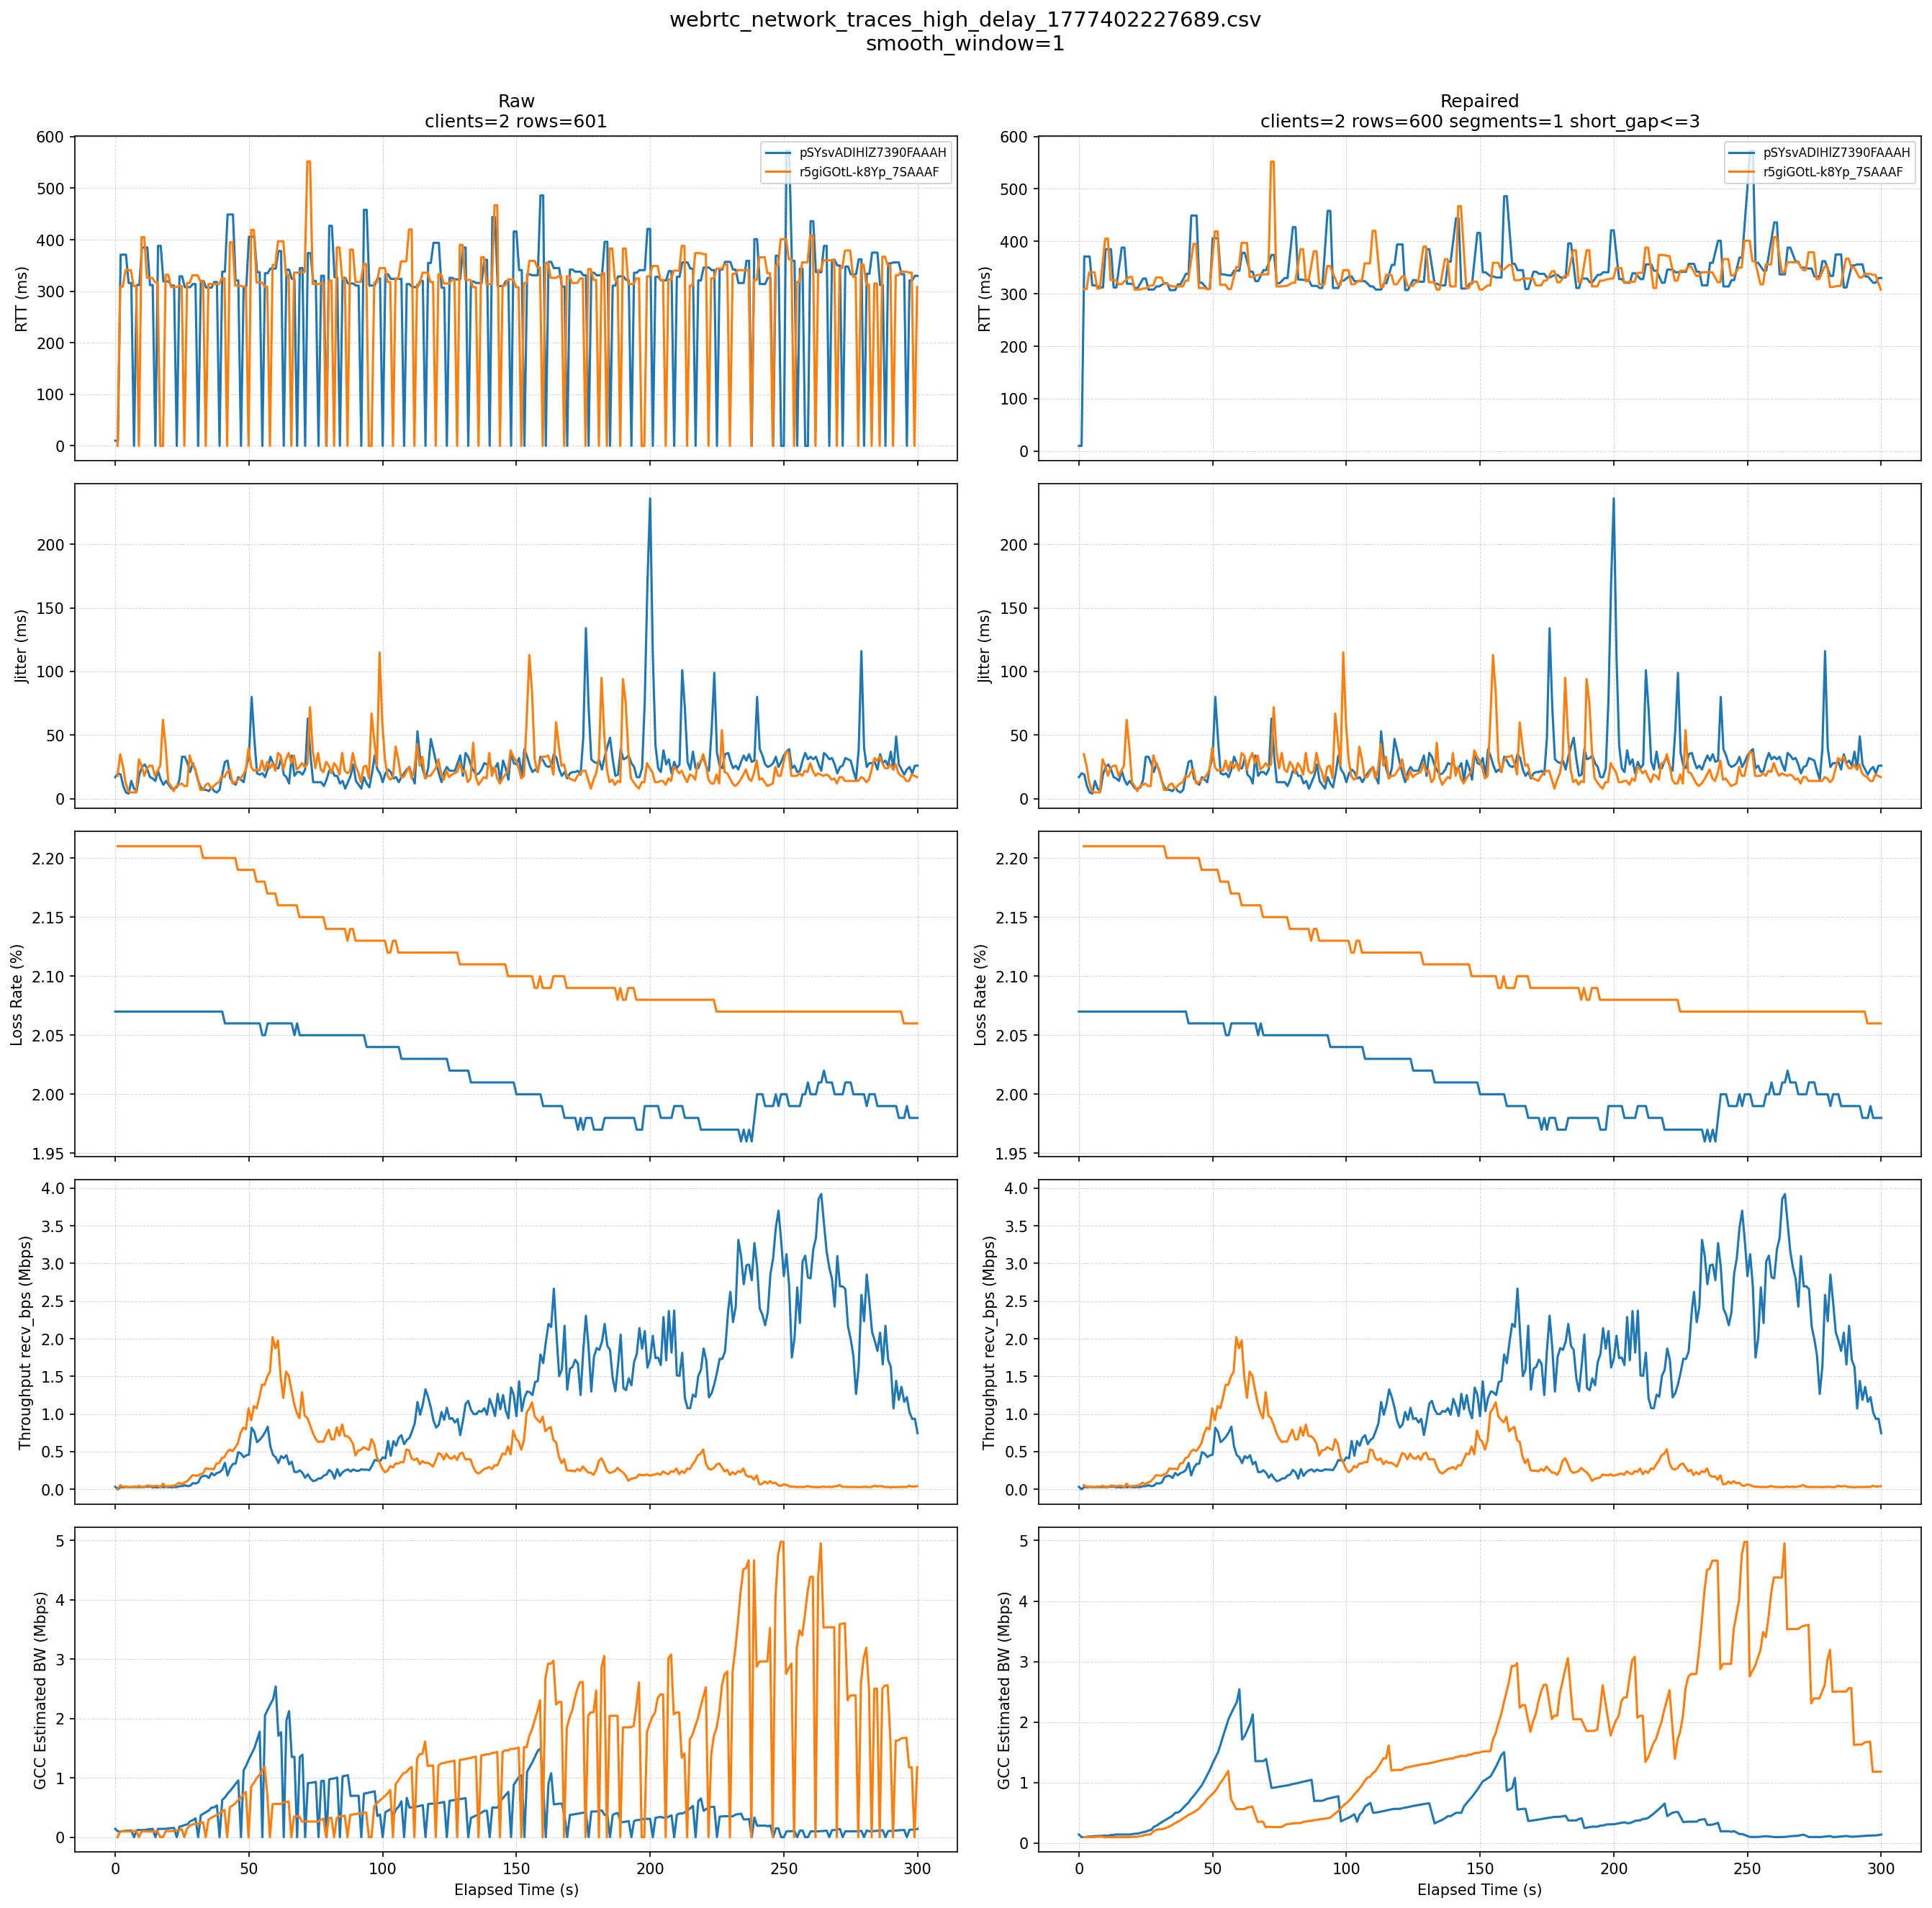
\includegraphics[width=\textwidth]{figures/traces/high_delay_trace_7689.png}
\subcaption{high\_delay}
\end{minipage}\hfill
\begin{minipage}{0.32\textwidth}
\centering
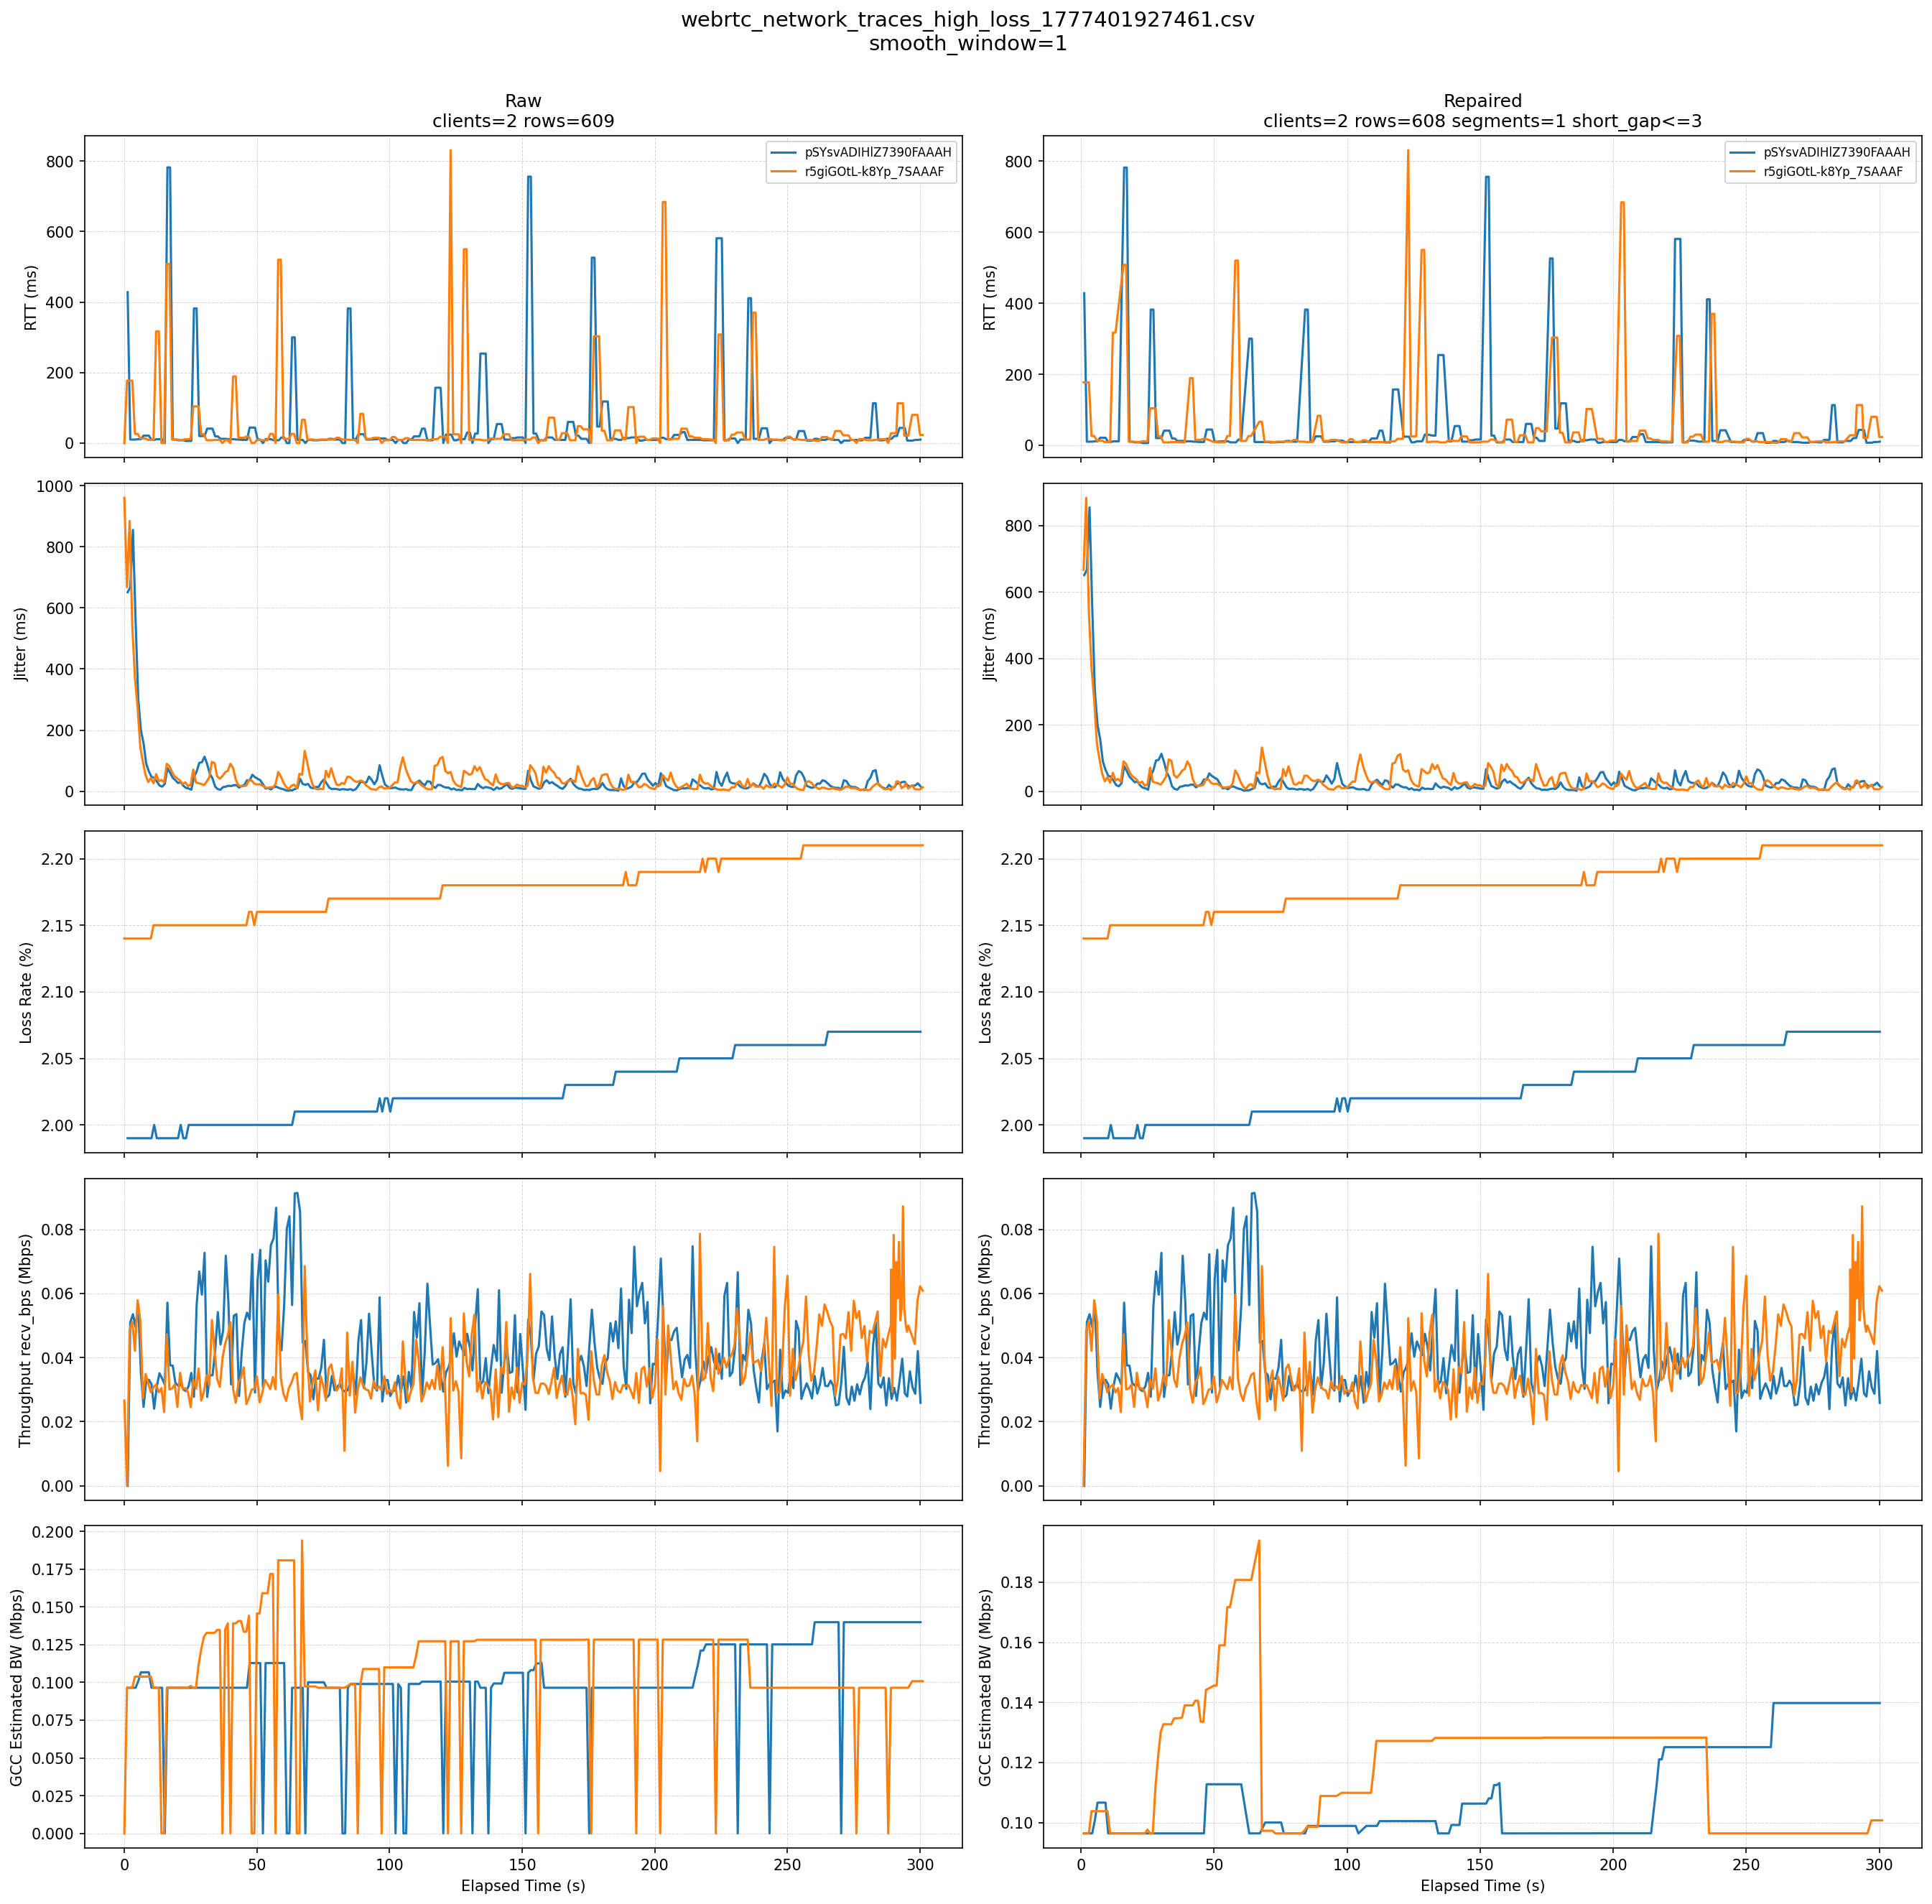
\includegraphics[width=\textwidth]{figures/traces/high_loss_trace_7461.png}
\subcaption{high\_loss}
\end{minipage}
\caption{典型场景下的原始/修复轨迹对比（二）}
\label{fig:traces-row2}
\end{figure}

\begin{figure}[htbp]
\centering
\begin{minipage}{0.32\textwidth}
\centering
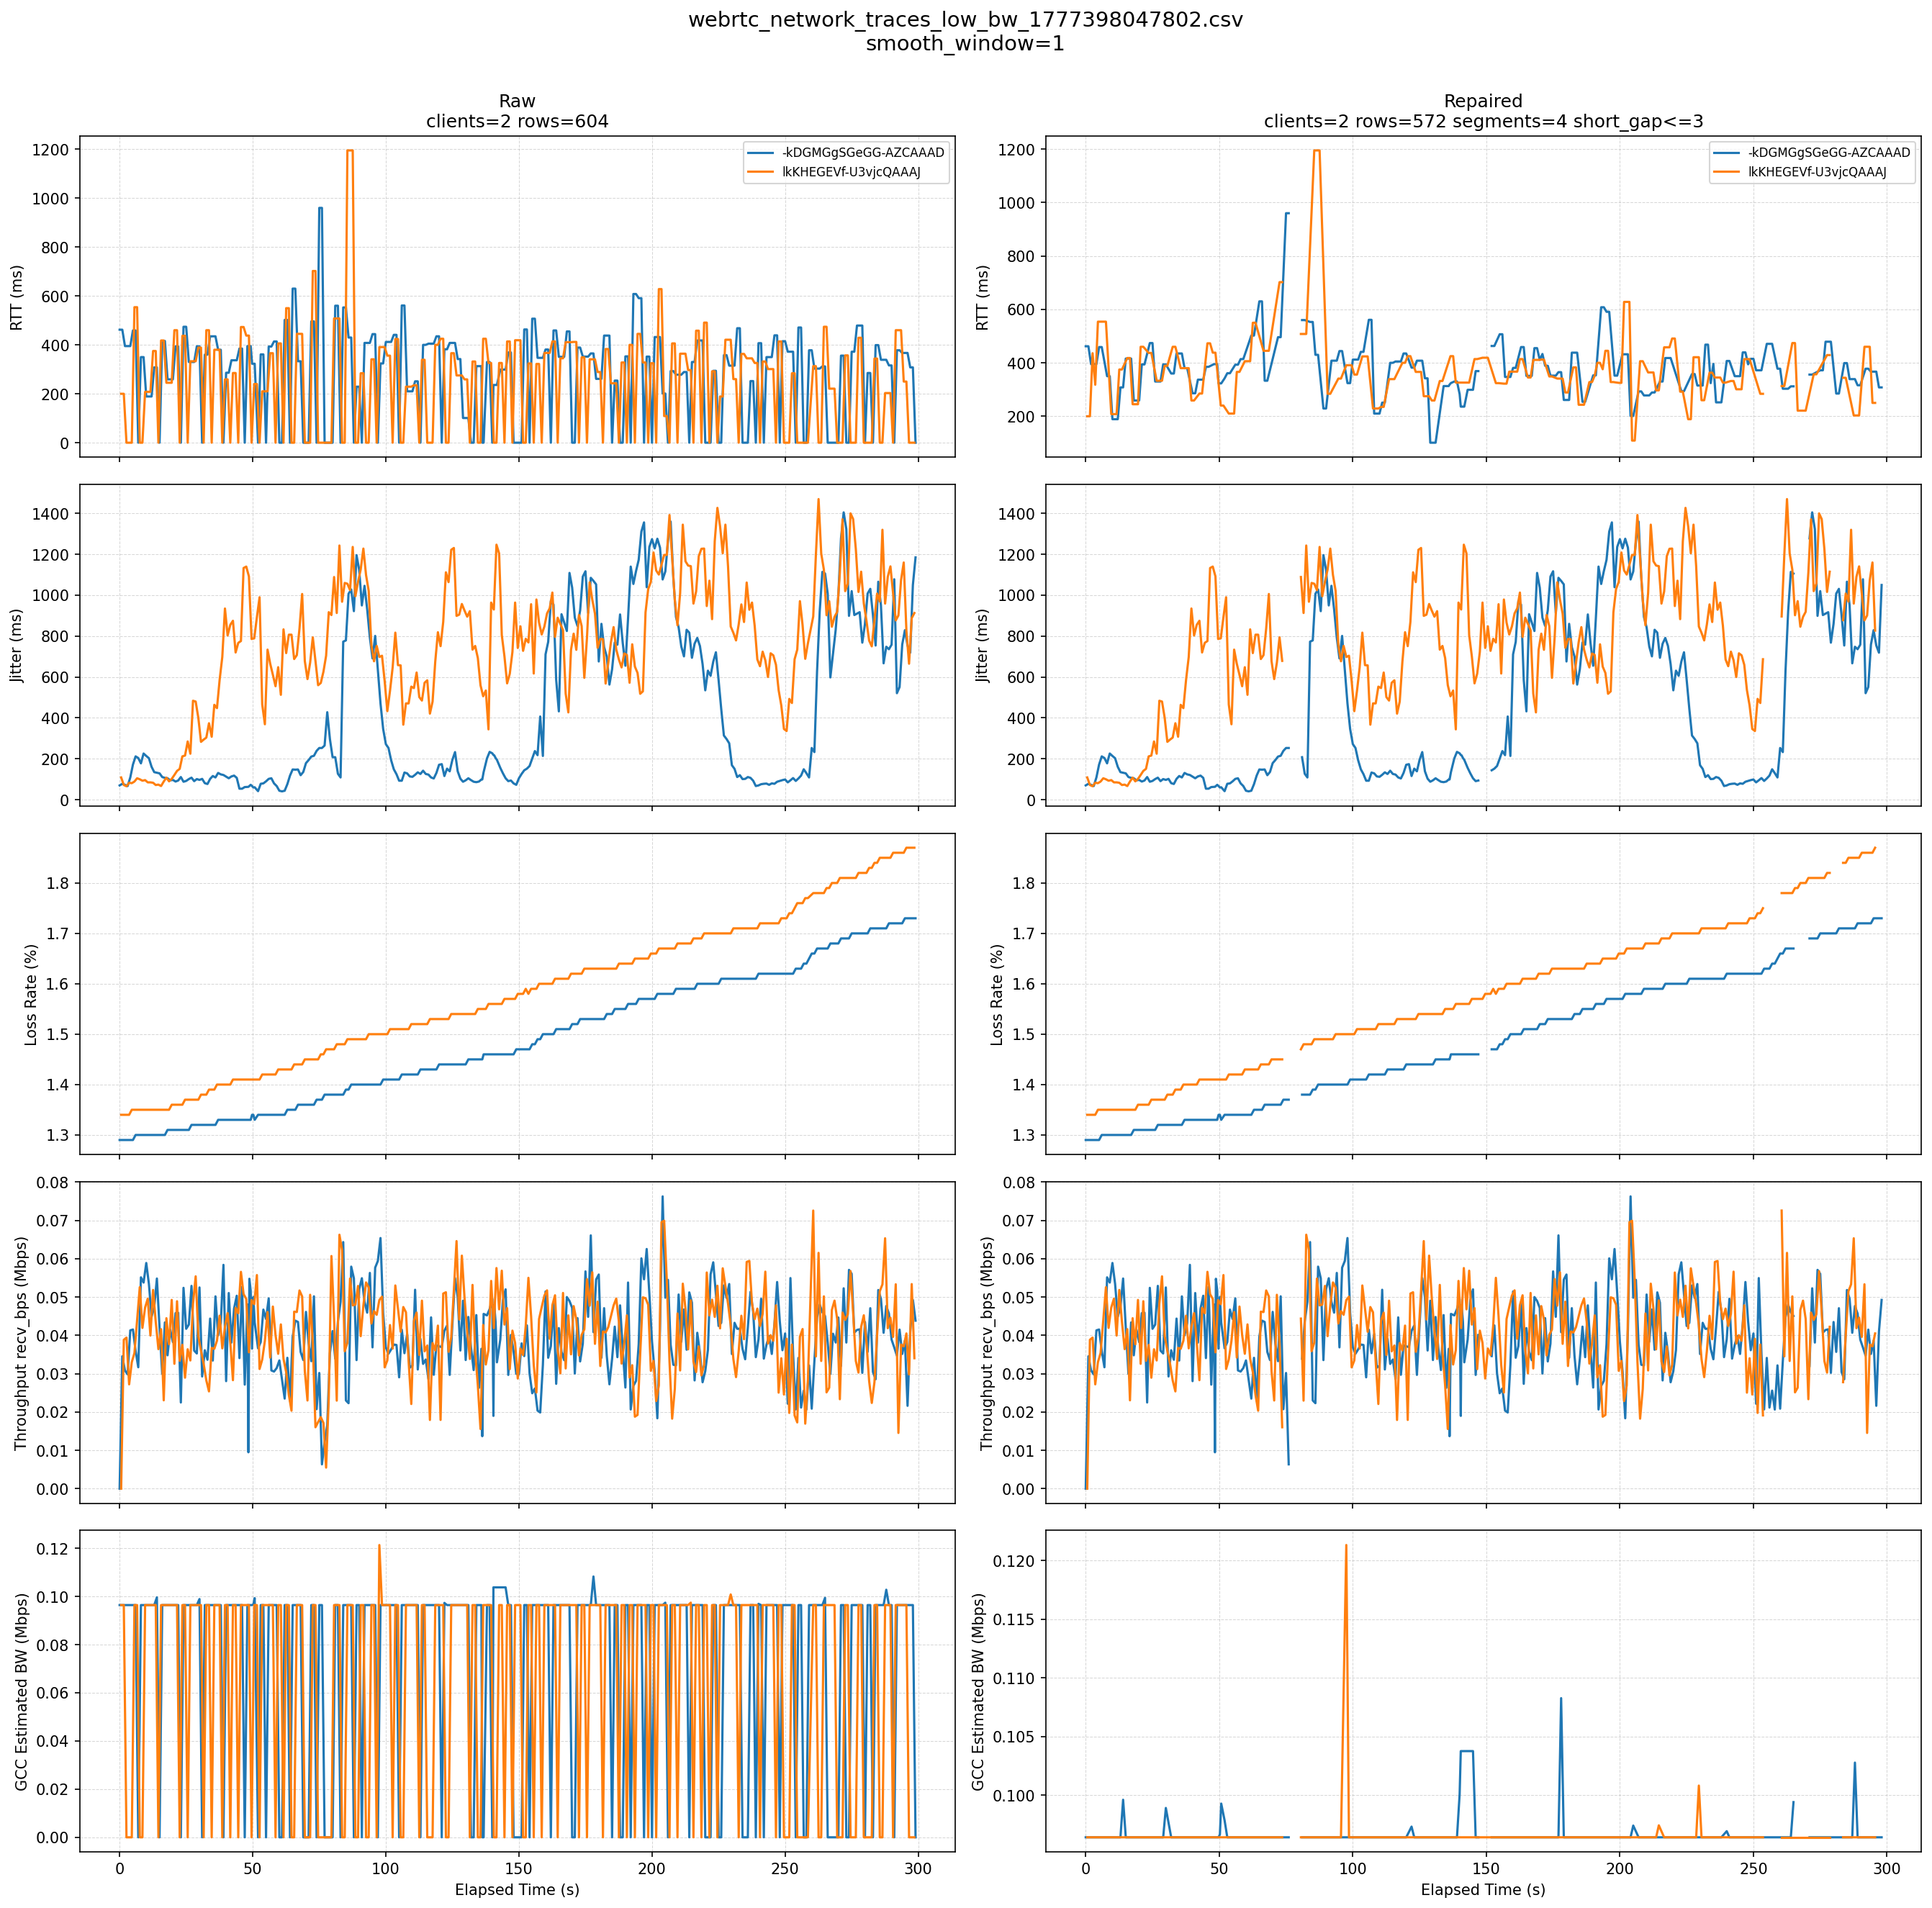
\includegraphics[width=\textwidth]{figures/traces/low_bw_trace_7802.png}
\subcaption{low\_bw}
\end{minipage}\hfill
\begin{minipage}{0.32\textwidth}
\centering
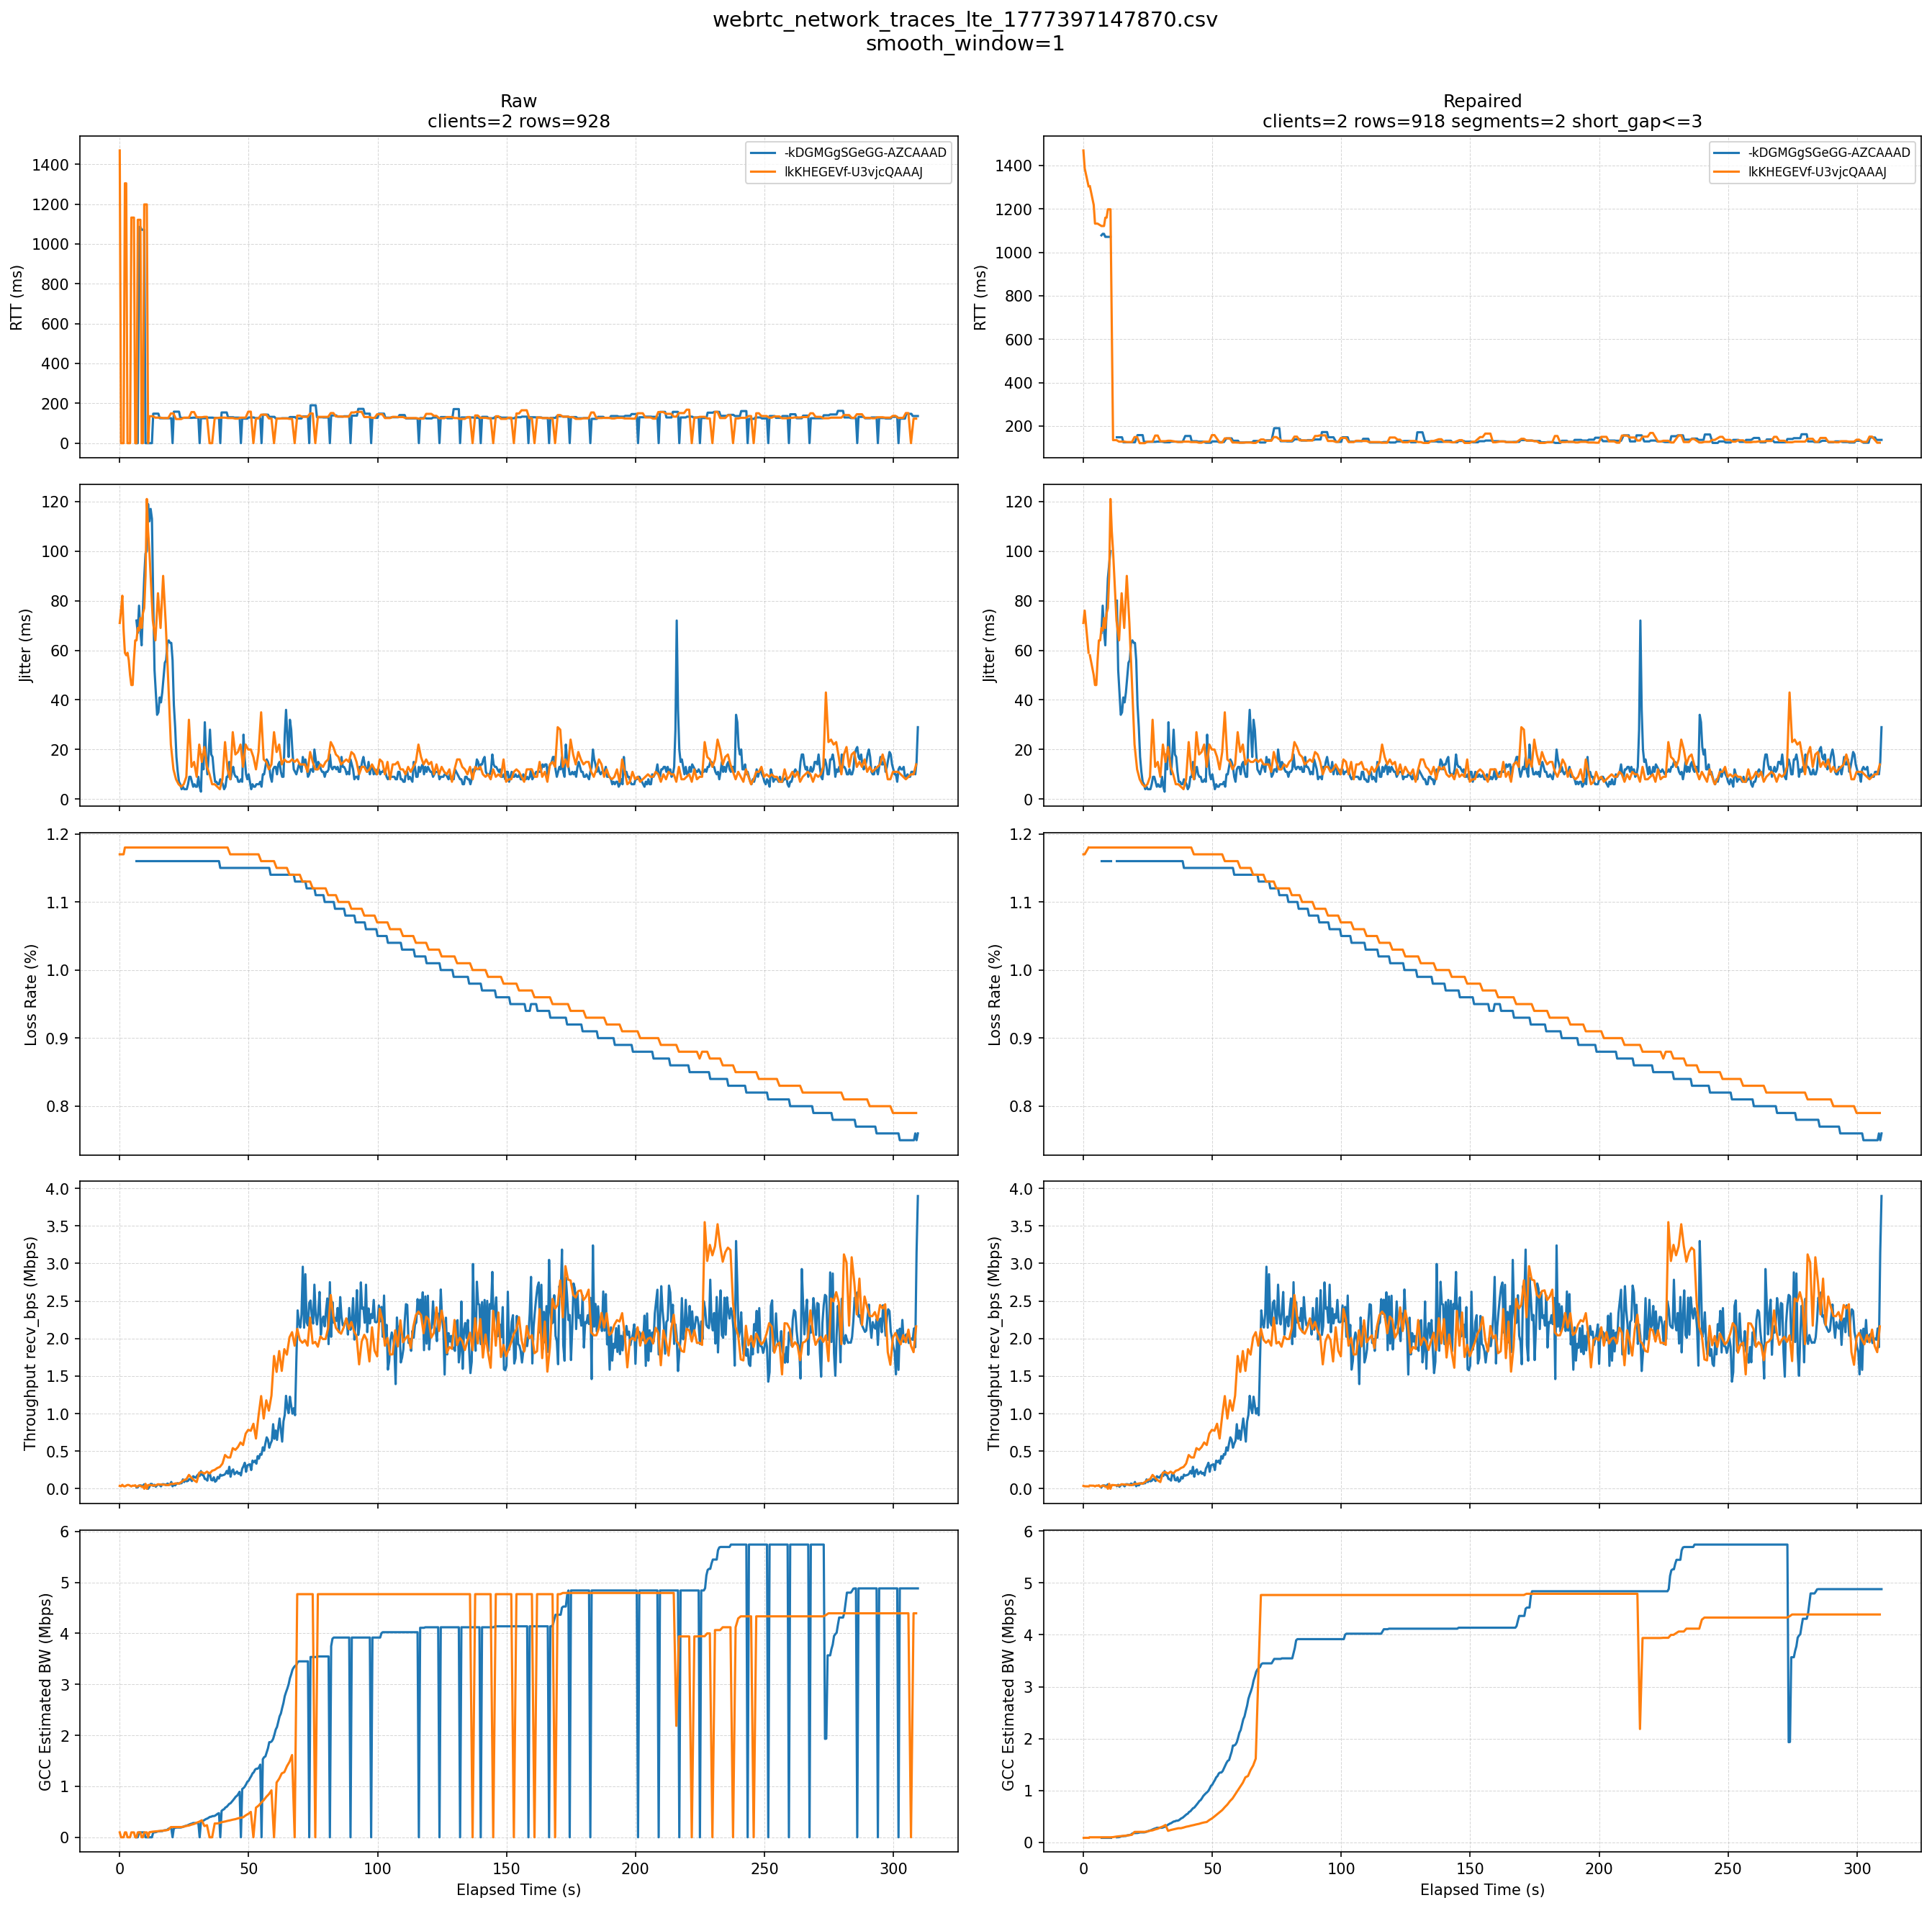
\includegraphics[width=\textwidth]{figures/traces/lte_trace_7870.png}
\subcaption{lte}
\end{minipage}\hfill
\begin{minipage}{0.32\textwidth}
\centering
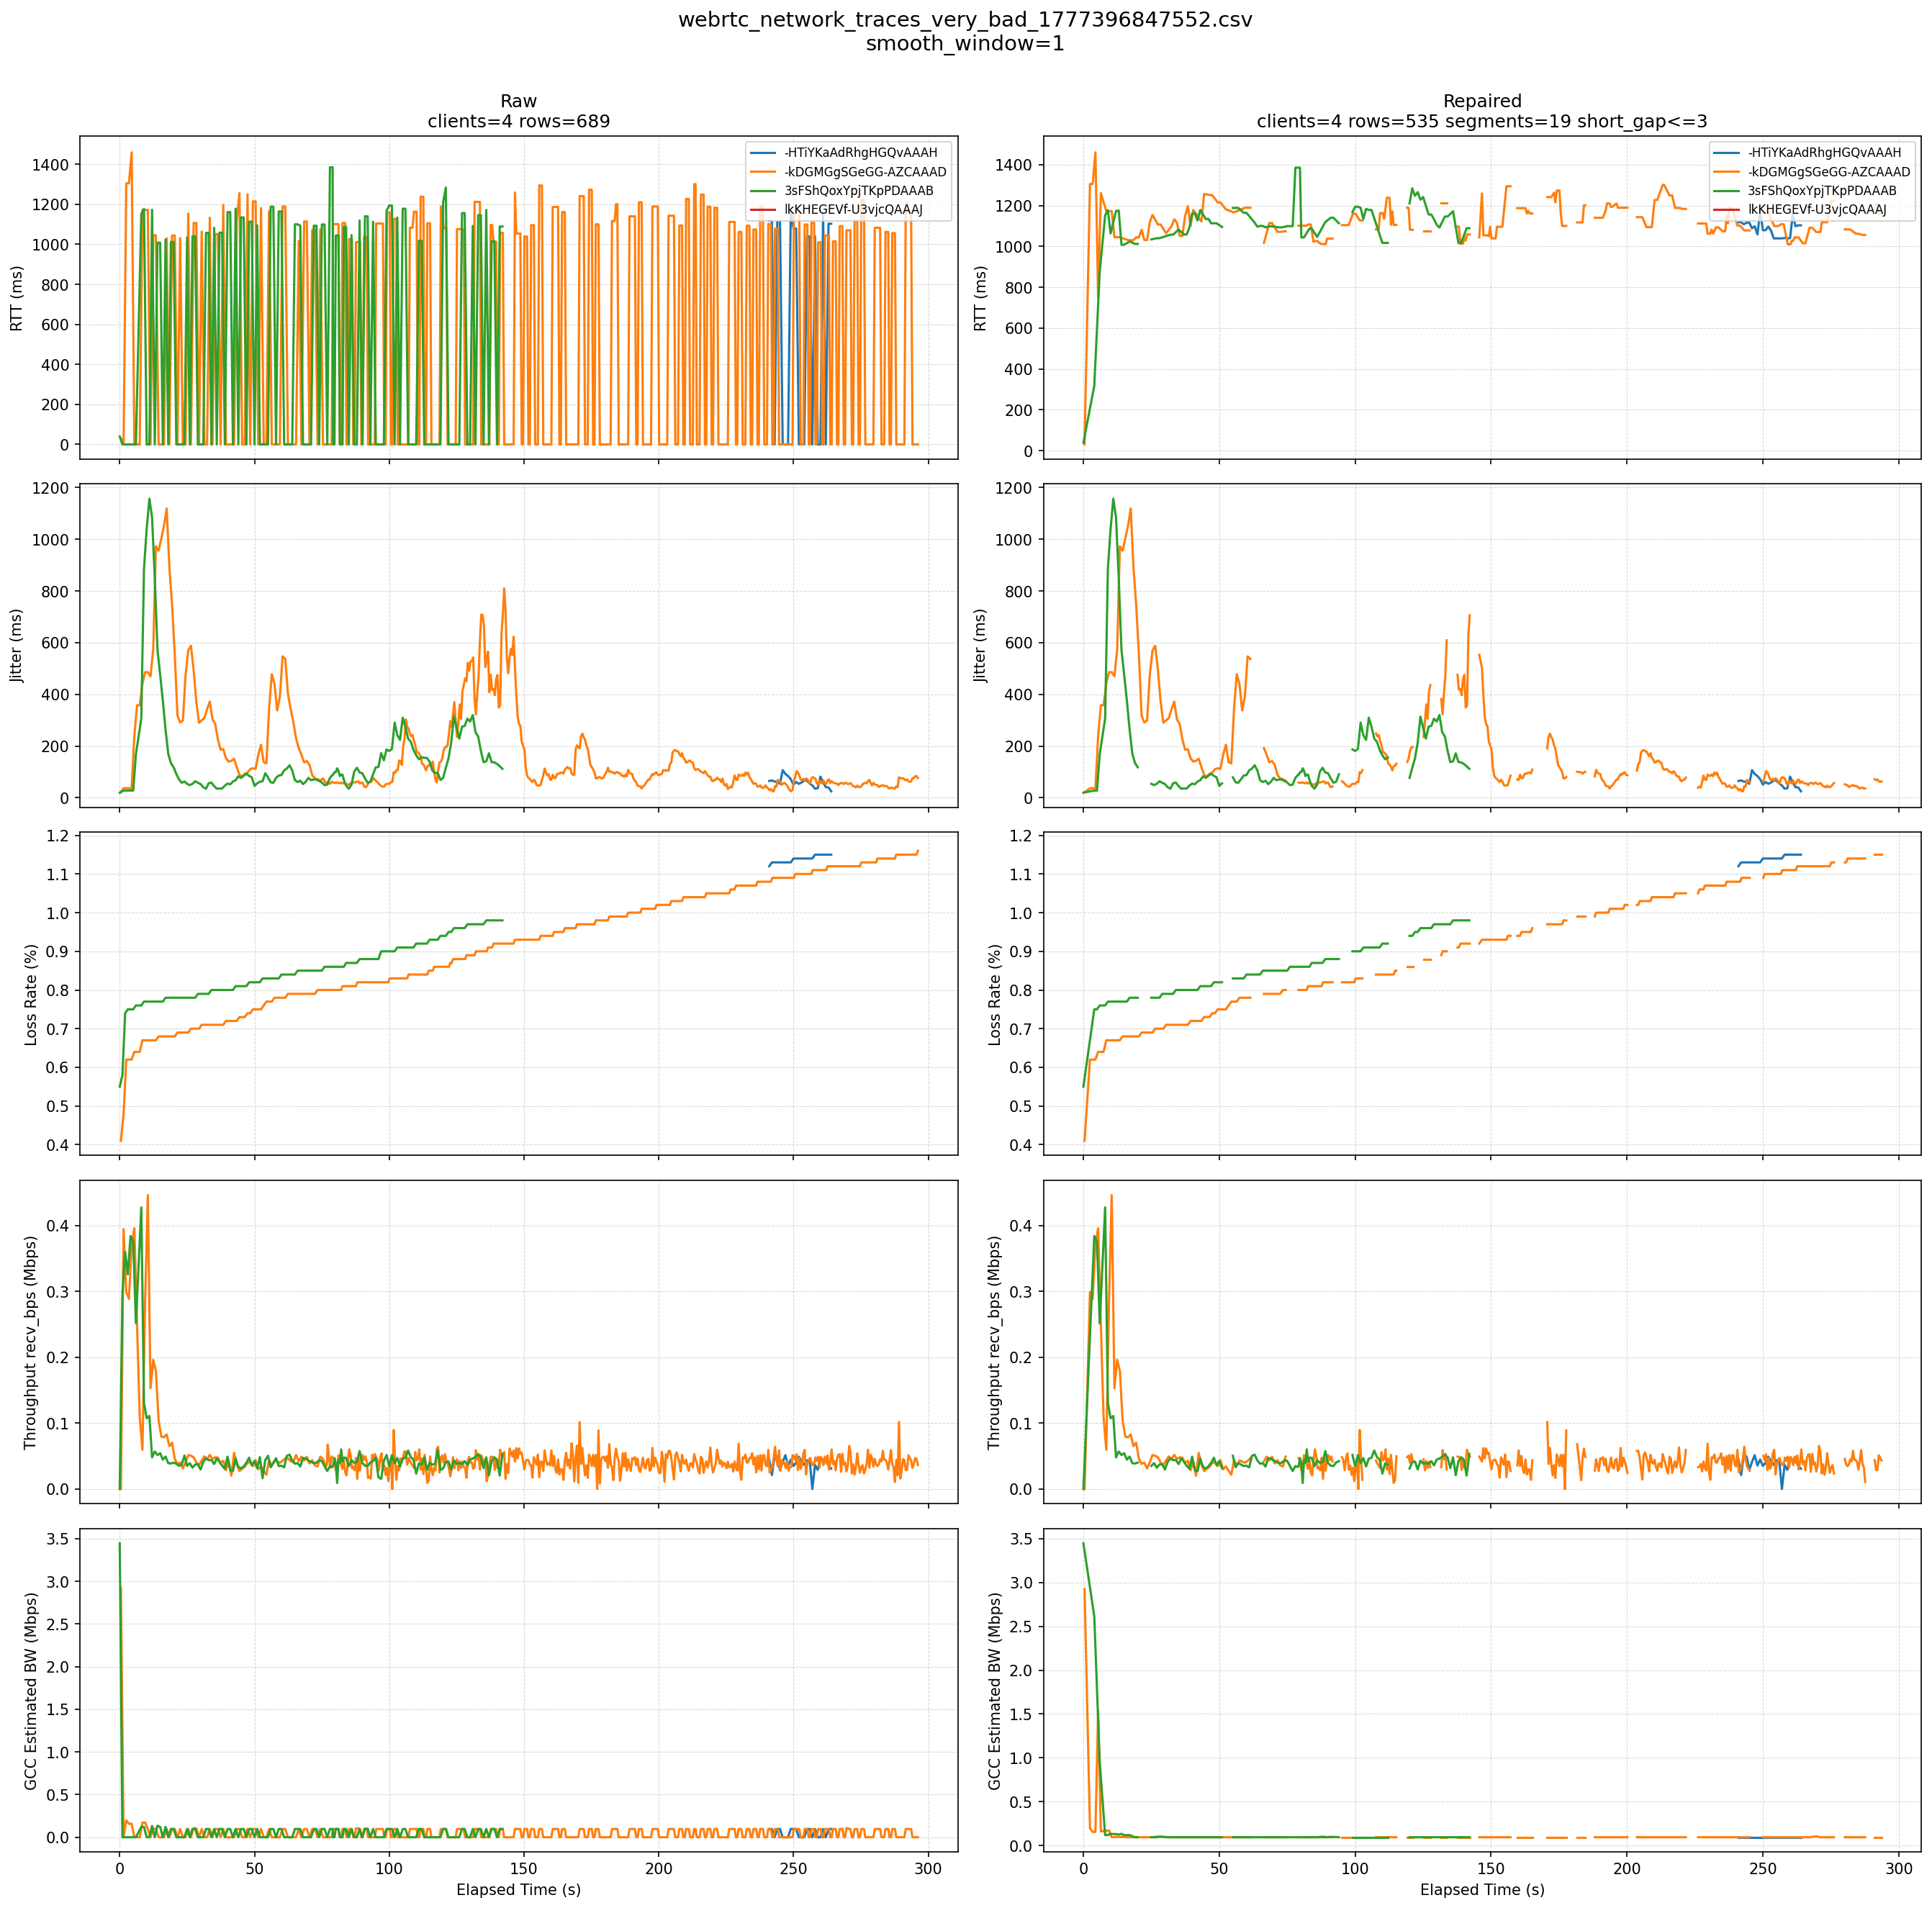
\includegraphics[width=\textwidth]{figures/traces/very_bad_trace_7552.png}
\subcaption{very\_bad}
\end{minipage}
\caption{典型场景下的原始/修复轨迹对比（三）}
\label{fig:traces-row3}
\end{figure}

\section{离线强化学习数据集的构建}
\label{sec:rl-dataset}

将 WebRTC 拥塞控制问题形式化为马尔可夫决策过程 $\mathcal{M} = \langle \mathcal{S}, \mathcal{A}, P, R, \gamma \rangle$ 时，需要为各组成元素赋予具体的网络语义。本文将状态空间 $\mathcal{S}$ 定义为最近十个采样周期内五维网络度量构成的滑动窗口向量，总维度为 $5 \times 10 = 50$；动作空间 $\mathcal{A}$ 定义为 GCC 算法在当前时刻输出的可用带宽估计 \texttt{estimated\_bw\_bps}，作为连续动作量；状态转移核 $P$ 由真实链路与 WebRTC 协议栈共同决定，属于未知环境动态；即时奖励 $R$ 基于下一时刻观测的网络质量指标计算；折扣因子 $\gamma$ 设为 $0.99$，体现对长期通信质量的关注。在离线强化学习框架下 $P$ 无需显式建模，学习算法仅从静态四元组中隐式提取价值与策略，因此构建高质量四元组成为本节的核心任务。

单一时刻的网络度量难以提供充分的决策信息。例如，孤立的 RTT $=50\,\text{ms}$ 无法判别延迟正在恶化抑或正在恢复。为此，本文采用滑动窗口机制构造状态向量：将时刻 $t$ 的状态 $s_t$ 取为从 $t-9$ 到 $t$ 共十个连续采样时刻、五个特征通道的二维窗口 $W_t \in \mathbb{R}^{5\times 10}$。窗口在送入策略网络前以特征优先（feature-major）方式展平为一维向量，即同一特征通道内的十个时间步在输出向量中保持连续：
\[
s_t = \big[\text{send\_bps}_{t-9:t},\ \text{recv\_bps}_{t-9:t},\ \text{rtt\_ms}_{t-9:t},\ \text{loss\_rate}_{t-9:t},\ \text{jitter\_ms}_{t-9:t}\big] \in \mathbb{R}^{50}.
\]
此种布局便于后续 GRU 编码器在每个特征通道上独立提取时序演化模式，再由全连接层完成跨通道特征融合。

奖励函数将多维网络质量目标压缩为标量信号。本文采用加权线性组合形式的 QoE 复合奖励，在执行动作 $a_t$ 后基于 $s_{t+1}$ 计算即时奖励：
\[
r_t = \alpha \cdot \log\!\Big(1 + \tfrac{\text{recv\_bps}_{t+1}}{10^6}\Big) - \beta \cdot \tfrac{\text{rtt\_ms}_{t+1}}{1000} - \gamma_l \cdot \text{loss\_rate}_{t+1} - \delta \cdot \tfrac{|a_t - a_{t-1}|}{10^6}.
\]
其中第一项以对数形式将接收吞吐量映射为视频质量正向激励；第二项将 RTT 缩放至秒级作为延迟惩罚，反映实时通话对端到端延迟的敏感性；第三项以丢包率作为质量退化惩罚；第四项对相邻动作的变化幅度施加弱惩罚，以抑制策略输出的剧烈振荡，避免因频繁码率切换导致编码器在关键帧与低质量帧之间反复跳转。本文将权重设为 $\alpha=\beta=\gamma_l=1.0$、$\delta=0.1$。

四元组的构建在清洗后的有效段上独立进行。具体流程为：在每个 \texttt{(clientId, segment\_id)} 分组内按时间戳升序排列后，自索引位置 $t = 9$ 起以步长一逐步滑动；对每个合法位置提取当前状态窗口、动作、前一动作（用于平滑惩罚）、下一状态窗口与即时奖励，并在段末位置置 \texttt{terminal=1}。当行内动作低于 $1\,\text{bps}$ 的极小阈值时该样本被丢弃，以排除 GCC 初始探测阶段产生的无效估计。由于切段已保证段内不存在 NaN，滑动窗口永不跨越数据断裂；同时严格按 \texttt{(clientId, segment\_id)} 分组也确保不同客户端、不同片段之间不共享窗口，从而使 IQL 训练中的 Bellman backup 不会跨越段边界进行错误的时序差分目标计算。

五维状态特征的原始量级跨越多个数量级——吞吐量典型值在 $10^5$–$10^7$ bps，RTT 在 $10$–$500$ ms，丢包率在 $[0,1]$，抖动在 $1$–$50$ ms。若不进行归一化，吞吐量分量将在输入层主导梯度，使价值与 Q 网络难以充分学习延迟与丢包对决策的影响。本文采用固定尺度缩放配合对称截断的归一化策略：缩放向量取 $\mathrm{scale}=[10^{-6}, 10^{-6}, 10^{-2}, 1.0, 10^{-2}]$，对每个特征通道独立缩放后将结果裁剪至 $[-10, +10]$ 区间。

最终产出的离线强化学习数据集以 NumPy 压缩存档形式持久化，包含归一化后的 \texttt{observations}、\texttt{next\_observations}、原始尺度的 \texttt{actions}、\texttt{rewards}、\texttt{terminals} 五个张量，并随附完整的归一化元信息以便推理端复现。同时，为支撑数据审查与异常回溯，构建脚本另产出一份带元信息的 CSV 与一份记录每个 \texttt{(scenario, trace, client, segment)} 组合贡献样本数的 manifest 统计表。基于完整采集与清洗流水线，本文最终获得 109{,}393 条有效 transition，覆盖 1{,}191 个连续有效段；动作空间分布范围为 $[9.24\times10^4,\ 1.13\times10^7]$ bps（均值约 $1.21\,\text{Mbps}$），奖励分布范围为 $[-1.65, +2.13]$（均值约 $0.155$）。该规模在网络拥塞控制领域已属可观，且行为策略 GCC 自身的探测—退避机制天然保证了从低带宽到高带宽的广泛状态覆盖，结合 IQL 通过期望回归仅依赖数据集中已有动作上界的保守性设计，使得该数据集足以支撑后续章节中策略网络的稳定训练与可靠泛化。

\section{本章小结}
\label{sec:chapter3-summary}

本章完整阐述了 WebRTC 专家策略数据集的采集、预处理与离线强化学习四元组构建方法。在数据采集链路层面，本文构建了以真实物理信道为承载、采集与评测严格物理隔离的实验平台，通过 \texttt{captureStream()} 实现一致的媒体源注入，通过周期性 \texttt{getStats()} 探针提取 RTT、抖动、丢包率、收发吞吐量与 GCC 预估带宽等核心特征，并以“场景—片段”双键索引落盘，保证轨迹的可溯源性。在专家数据收集与预处理层面，本文以 GCC 作为行为策略，在九类参数化网络环境下采集得到具有代表性的原始轨迹，并针对真实采集中普遍存在的周期性零点、短暂缺失与长期断裂三类缺陷设计了“异常标记—短缺失插值—长断裂切段”三级清洗流程，配合全样本可视化审查保证了数据的物理可信度。在离线强化学习数据集构建层面，本文将拥塞控制问题形式化为 MDP，采用十步滑动窗口构造五十维状态、以 GCC 输出作为动作、以包含吞吐对数收益与延迟、丢包、动作平滑惩罚的复合 QoE 函数作为奖励，并以固定尺度缩放配合对称截断的归一化策略保证训练—推理一致性。最终产出的 109{,}393 条有效 transition 数据集，为后续章节中基于 IQL 的策略训练与对照实验奠定了坚实的工程基础。
